\documentclass{article}
%
%
%	vector_calculus.tex
%
%	David Meyer
%	dmm613@gmail.com
%	05 Sep 2022
%
%
%   get various packages
%
\usepackage[margin=1.0in]{geometry}                                     % adjust margins
\geometry{letterpaper}                                                  % or a4paper or a5paper or ... 
\usepackage{url}                                                        % need this to use URLs in bibtex
\usepackage{setspace}                                                   % need this for \setstrech{...}
\usepackage{scrextend}                                                  % need this for addmargin
\usepackage[export]{adjustbox}                                          % need this to get frame for includegraphics
%
%   tikz et al
%
\usepackage{tikz}
\usetikzlibrary{calc,patterns,angles,quotes,shapes,math,decorations,
                through,intersections,lindenmayersystems,backgrounds,
                hobby}
\tikzset{>=latex}                                                       % default to LaTeX arrow head
\usepackage{circuitikz}                                                 % draw circuits    
\usepackage{pgfplots}
%
%	more math stuff
%
\usepackage{amsmath,amsfonts,amssymb,amsthm}
\usepackage{mathtools}
\usepackage{commath}                                                    % get \norm{x}
\usepackage{fixmath}                                                    % get \mathbold
\usepackage{gensymb}                                                    % get \degree
\usepackage{mathrsfs}
\usepackage{hyperref}
\usepackage{subcaption}
\usepackage{authblk}
\usepackage{graphicx}
\usepackage{hyperref}
\usepackage{alltt}
\usepackage{color}
\usepackage{float}
\usepackage{braket}
\usepackage{siunitx}
\usepackage{relsize}
\usepackage{multirow}
\usepackage{esvect}
%
%	watermarks
%
% \usepackage{draftwatermark}
% \SetWatermarkText{Draft}
% \SetWatermarkScale{5}
% \SetWatermarkLightness {0.9} 
% \SetWatermarkColor[rgb]{0.7,0,0}
%
%
%	theorems, definitions, etc
%
\theoremstyle{definition}
\newtheorem{theorem}{Theorem}[section]
\newtheorem{definition}{Definition}[section]
\newtheorem{proposition}{Proposition}[section]
\newtheorem{lemma}{Lemma}[section]
\newtheorem{example}{Example}[section]
\newtheorem{remark}{Remark}[section]
%
%	The following code allows you to do
%
%	\begin{bmatrix}[r] (or [c] or [l])
%
\makeatletter
\renewcommand*\env@matrix[1][c]{\hskip -\arraycolsep
  \let\@ifnextchar\new@ifnextchar
  \array{*\c@MaxMatrixCols #1}}
\makeatother
%
%	make \arg{min,max}_{n \to \infty} work nicely
%
\newcommand{\argmax}{\operatornamewithlimits{argmax}}
\newcommand{\argmin}{\operatornamewithlimits{argmin}}
%
%	handy commands
%
\newcommand*{\Scale}[2][4]{\scalebox{#1}{$#2$}}
\DeclareMathOperator{\E}{\mathbb{E}}
\DeclareMathOperator{\bda}{\Big \downarrow}						% big down arrow
\newcommand{\veq}{\mathrel{\rotatebox{90}{$=$}}}
%
%	Title, author and date
%
\title{A Few Notes on Vector Calculus }
\author{David Meyer \\ \href{mailto:dmm613@gmail.com}
                            {dmm613@gmail.com}}
\date{Last update: \today}
%
%	be compatible
%
\pgfplotsset{compat=1.17} 
%
%
%
\begin{document}
\maketitle
%
%
%
\section{Vector Spaces}
\subsection{Definitions}

\begin{definition}A \emph{field} is an algebraic structure\footnote{See Appendix A
for a brief review of a few important algebraic structures.} consisting 
of a non-empty set $\mathbb{K}$ equipped with two binary operations, $+$ 
(addition) and $\cdot$ (multiplication), satisfying the conditions\footnote{See 
Appendix B for more on groups and fields.}:

\medskip
\begin{itemize}
\item [] (A) $(\mathbb{K},+)$ is an Abelian group with identity element $0$ 
             (called zero).
\item [] (M) $(\mathbb{K} \backslash \{0\}, \cdot)$ is an Abelian group with 
             identity element 1.
\item [] (D) The distributive law $a(b+c)=ab+ac$ holds for all $a,b,c \in \mathbb{K}$.
\end{itemize}

\medskip
\noindent
Examples of important fields include

\medskip
\begin{itemize}
\item $\mathbb{Q}$,     the field of rational numbers
\item $\mathbb{R}$,     the field of real numbers
\item $\mathbb{C}$,     the field of complex numbers
\item $\mathbb{Z}_{p}$, the field of integers mod $p$ for prime $p$ 
\end{itemize}
\end{definition}

\smallskip
\begin{definition}
A vector space $V$ over a field $\mathbb{K}$ is an algebraic structure consisting 
of a non-empty \\ set $V$ equipped with a binary operation $+$ (vector addition) 
and a scalar multiplication operation \\
$(a,v) \in \mathbb{K} \times V \mapsto av \in V$
such that the following rules hold:


\bigskip
\noindent
(VA) $(V,+)$ is an Abelian group with identity element $\mathbf{0}$ (the zero vector). 

\bigskip
\noindent
(VM) Rules for scalar multiplication:

\medskip
\begin{itemize}
\item [] (VM0) Closure: For any $a   \in \mathbb{K}$ and $v \in V$ there is a unique element $av \in V$.
\item [] (VM1) $\text{Distributivity}_{1}$: For any $a \in \mathbb{K}$ and $u,v \in V$ we have $a(u+v)=au+av$.
\item [] (VM2) $\text{Distributivity}_{2}$: For any $a,b \in \mathbb{K}$ and $v \in V$ we have $(a+b)v=av+bv$.
\item [] (VM3) Associativity: For any $a,b \in \mathbb{K}$ and $v \in V$ we have $(ab)v=a(bv)$.
\item [] (VM4) Identity: For any $v \in V$ we have $1v = v$ (where $1$ is the identity element of $\mathbb{K}$).
\end{itemize}
\end{definition}

\medskip
\noindent
Since vector spaces have two kinds of elements, namely elements of $\mathbb{K}$ and 
elements of $V$, we distinguish them by calling the elements of $\mathbb{K}$ scalars 
and the elements of $V$ vectors.

\bigskip
\noindent
A vector space over the field $\mathbb{R}$ is often called a real vector space 
while a vector space over $\mathbb{C}$ is called a complex vector space.

\subsection{Vectors}
In this section we'll define the vector notation that we will use in these
notes as well as a few important vector operations.

\smallskip
\subsubsection{Notation} 

\medskip
\noindent
In these notes we will use boldface to represent a vector.
Specifically, we will use $\mathbf{a} = (a_1,a_2,\hdots, a_n)$ 
to represent a column or row vector in some $n$-dimensional
space (usually $\mathbb{R}$ or $\mathbb{C}$). If $\mathbf{a}$ 
is a column vector then in matrix format

\begin{flalign*}
\mathbf{a} = 
\underbrace {
\begin{bmatrix} 
a_1 \\
a_2 \\
\vdots \\
a_n
\end{bmatrix}}_{n \times 1}
\end{flalign*}


\medskip
\noindent
Alternatively, if $\mathbf{a}$ is a row vector then
in matrix format

\begin{flalign*}
\mathbf{a} = 
\underbrace{
\begin{bmatrix} 
a_1 \; a_2 \; \hdots \; a_n
\end{bmatrix}}_{1 \times n}
\end{flalign*}

\bigskip
\noindent
The \emph{transpose} of a vector $\mathbf{a}$,
$\mathbf{a}^{\intercal}$, is defined as follows: 
If $\mathbf{a}$ is a column vector then

\begin{flalign*}
\mathbf{a}^{\intercal} = 
\begin{bmatrix} 
a_1 \; a_2 \; \hdots \; a_n
\end{bmatrix}
\end{flalign*}

\smallskip
\noindent
Alternatively, if $\mathbf{a}$ is a row vector then

\begin{flalign*}
\mathbf{a}^{\intercal} = 
\begin{bmatrix} 
a_1 \\
a_2 \\
\vdots \\
a_n
\end{bmatrix}
\end{flalign*}


\bigskip
\noindent
Adding a "hat" to a vector denotes the unit 
vector. That is, for a vector $\mathbf{u}$, 
$\hat{\mathbf{u}}$ is defined to be 

\medskip
\begin{equation}
\hat{\mathbf{u}} := \dfrac{\mathbf{u}}{\| \mathbf{u} \|}
\label{eqn:hat}
\end{equation}

\bigskip
\noindent
where $\norm{\mathbf{u}}$ is the Euclidean Norm
of the vector $\mathbf{u}$ (Definition \ref{def:euclidean_norm}).

\bigskip
\noindent
In words: $\hat{\mathbf{u}}$ is a vector of unit
length in the $\mathbf{u}$ direction. 

\bigskip
\noindent
Similarly, $\mathbf{\hat{i}}$, $\mathbf{\hat{j}}$, and
$\mathbf{\hat{k}}$ are unit vectors in $\mathbb{R}^3$ in the $x$,
$y$, and $z$ directions respectively. Note that
$\mathbf{\hat{i}}$, $\mathbf{\hat{j}}$, and $\mathbf{\hat{k}}$
are the canonical basis vectors for $\mathbb{R}^3$
\cite{notes:basis} and have column vector format

\bigskip
\begin{equation*}
{\displaystyle \mathbf {\hat {i}} 
= {\begin{bmatrix}1\\0\\0\end{bmatrix}},\,\,
\mathbf {\hat {j}} = {\begin{bmatrix}0\\1\\0\end{bmatrix}},\,\,
\mathbf {\hat {k}} = {\begin{bmatrix}0\\0\\1\end{bmatrix}}}
\end{equation*}

\medskip
\bigskip
\noindent
I have also seen $\mathbf{e}_i$ used to represent the $i^{th}$
basis vector in $\mathbb{R}^n$. So $\mathbf{e}_i$ is a vector
with a one in the $i^{th}$ position and a zero in each of the
other $n - 1$ positions.  In $\mathbb{R}^3$ this means that
$\mathbf{e}_1 = \mathbf{\hat{i}}$, $\mathbf{e}_2 =
\mathbf{\hat{j}}$, and $\mathbf{e}_3 = \mathbf{\hat{k}}$.


\bigskip
\noindent
In general, the standard basis (which is sometimes called the
computational basis) for the $n$-dimensional Euclidean space
consists of the ordered set of $n$ distinct vectors

\medskip
\begin{equation*}
\{\mathbf {e} _{i}: 1 \leq i \leq n\}
\end{equation*}

\bigskip
\noindent
where $\mathbf{e}_i$ is the $i^\text{th}$ basis vector, that is,
it has a one in the $i^\text{th}$ coordinate (position) and zeros
everywhere else\footnote{This is called a "one-hot"
encoding in machine learning, where the $i$'s might be
the classes in a classification problem.}. The $\mathbf{e}_i$ have
column vector format

\begin{flalign*}
\mathbf{e}_{1} = 
\begin{bmatrix} 
1 \\
0 \\
\vdots \\
0 \\
0
\end{bmatrix} \!\! , \;
\mathbf{e}_{2} = 
\begin{bmatrix} 
0 \\
1 \\
\vdots \\
0 \\
0
\end{bmatrix} \!\! , 
\hdots  , \; 
\mathbf{e}_{n-1} =
\begin{bmatrix} 
0 \\
0 \\
\vdots \\
1 \\
0
\end{bmatrix} \!\! , \;
\mathbf{e}_{n} =
\begin{bmatrix} 
0 \\
0 \\
\vdots \\
0 \\
1
\end{bmatrix}
\end{flalign*}


\bigskip
\noindent
Using these definitions we can define the parametric form of some
curve $C$ in $\mathbb{R}^3$, $\mathbf{r}(t)$, as follows:

\medskip
\begin{equation*}
\mathbf{r}(t) = g(t) \mathbf{\hat{i}} +h(t)
\mathbf{\hat{j}} + k(t) \mathbf{\hat{k}}
\end{equation*}

\bigskip
\noindent
where $t \in [a,b]$ and $g(t)$, $h(t)$, and $k(t)$ are scalar
functions\footnote{A scalar function is a function $f$ such that
$f: \mathbb{R}^n \to \mathbb{R}$.}.


\bigskip
\noindent
Another common notation for vectors is $\vec{r}(t)$, where
$\vec{r}(t)$ might be defined as follows:


\bigskip
\begin{equation*}
\vec{r}(t) = g(t) \hat{i} +h(t) \hat{j} + k(t) \hat{k} 
\end{equation*}


\subsubsection{A Few Vector Operations}

\bigskip
\begin{definition}
{\bf Inner Product:} $\langle \mathbf{a}, \mathbf{b} \rangle$

\bigskip
\noindent
The inner product (aka dot product 
or scalar product) of two $n$-dimensional vectors 
$\mathbf{a} = (a_1,a_2,\hdots, a_n)$ and 
$\mathbf{b} = (b_1,b_2,\hdots, b_n)$, usually 
denoted by either $\langle \mathbf{a}, \mathbf{b} 
\rangle$ or $\mathbf{a} \cdot \mathbf{b}$,
is defined to be the scalar value

\medskip
\begin{equation}
\langle \mathbf{a}, \mathbf{b} \rangle := \sum\limits_{j = 1}^{n} a_j b_j
\label{eqn:inner}
\end{equation}
\end{definition}

\smallskip
\noindent
Since $a_j$ and $b_j$ are scalars (and scalar multiplication commutes)
the inner product commutes:

\bigskip
\begin{equation}
  \langle \mathbf{a}, \mathbf{b} \rangle
  = \sum\limits_{j = 1}^{n} a_j b_j
  = \sum\limits_{j = 1}^{n} b_j a_j
  =  \langle \mathbf{b}, \mathbf{a} \rangle 
\label{eqn:dot_reverse}
\end{equation}

\bigskip
\noindent
It is worth noting that there are some cases in which the dot notation
is used but the operation does not commute. For example, the \emph{divergence} 
of $\mathbf{A}$, is defined to be div $\mathbf{A} = \nabla \cdot \mathbf{A}$ 
\cite{the_role_of_grad}. Here the operation denoted by $\cdot$ is "reminiscent" 
of the inner product (as defined in Equation (\ref{eqn:inner})) but does not commute. 
That is


\begin{equation}
\nabla \cdot \mathbf{A} \neq \mathbf{A} \cdot \nabla
\label{eqn:dot_does_not_commute}
\end{equation}

\bigskip
\noindent
One way to see this is to notice that the LHS of Equation 
(\ref{eqn:dot_does_not_commute}) is a scalar function while
the RHS  is a differential operator.

\bigskip
\noindent
If $\mathbf{a}$ and $\mathbf{b}$ are column vectors then their
inner product $\langle \mathbf{a}, \mathbf{b} \rangle$ can also be 
written as the matrix product $\mathbf{a}^{\intercal}\mathbf{b}$. 
Similarly, if $\mathbf{a}$ and $\mathbf{b}$ are row vectors then 
their inner product can be written as the matrix product
$\mathbf{a}\mathbf{b}^{\intercal}$. For example, the inner product
of two $n \times 1$ column vectors $\mathbf{a}$ and $\mathbf{b}$
is equivalent to the following matrix multiplication:


\begin{flalign*}
  \langle \mathbf{a}, \mathbf{b}\rangle  = \mathbf{a}^{\intercal}\mathbf{b} = 
  \begin{bmatrix} a_1 \; a_2 \; \hdots \; a_n \end{bmatrix} 
  \begin{bmatrix} b_1 \\ b_2 \\ \vdots \\ b_n \end{bmatrix} = 
  \sum\limits_{j = 1}^{n} a_j b_j
\end{flalign*}



\medskip
{\setstretch{1.5}									% get a bit of extra space
\noindent
According to the Pythagorean theorem, the length of a vector
$\mathbf{a} = (a_1,a_2,a_3) \in \mathbb{R}^3$, denoted
$\|\mathbf{a} \|$, equals $\sqrt{a_1^2 + a_2^2 + a_3^2}$. The
next definition is a generalization of the notion of length to
vectors in $\mathbb{R}^n$.
\par}


\bigskip
\begin{definition}
\label{def:euclidean_norm}
{\bf Euclidean Norm:} $\|\mathbf{x}\|$


\bigskip
\noindent
The Euclidean norm of a vector $\mathbf{x} = (x_1,x_2,\ldots, x_n) \in \mathbb{R}^{n}$
is defined to be

\smallskip
\begin{equation}
\|\mathbf{x}\| := \sqrt{\langle \mathbf{x}, \mathbf{x}} \rangle =
\sqrt{\sum\limits_{j = 1}^{n} x_{j}^{2}}
\label{eqn:magnitude}
\end{equation}
\end{definition}

\smallskip
\begin{definition}
\label{def:p_norm}
{\bf $p$-Norm:} ${\norm{\mathbf {x}}}_{p}$


\bigskip
\noindent
The $p$-norm of a vector $\mathbf{x} = (x_{1},x_{2}. \ldots , x_{n})$
is defined to be

\smallskip
\begin{equation*}
{\norm{\mathbf {x}}}_{p} := {\left(\sum _{i=1}^{n} 
	{\left | x_{i} \right |}^{p}\right)}^{1/p}
\end{equation*}

\noindent
for $p \geq 1$ and $p \in \mathbb{R}$. 

\bigskip
\setstretch{1.25}
\noindent
For $p = 1$, we get the taxicab norm, for $p = 2$ we get the
Euclidean norm, and as $p$ approaches $\infty$ the $p$-norm
approaches the infinity norm or maximum norm: ${\displaystyle
{\norm{\mathbf {x}}}_{\infty } :=\max
_{i}\left|x_{i}\right|}$.
\end{definition}

\noindent
The inner product also has an interesting geometric interpretation:



\smallskip
\begin{theorem} {$\langle \mathbf{x}, \mathbf{y} \rangle = 
\norm{\mathbf{x}} \norm{\mathbf{y}}\cos \theta$}
\label{theorem:ip}

\medskip
{\setstretch{1.25}
\noindent 
{\bf Proof.} Assume that 
$\mathbf{x}$ and $\mathbf{y}$ are two linearly independent vectors in 
$\mathbb{R}^3$ and that $M$ is the plane generated by them. Then $\mathbf{x}$ 
and $\mathbf{y}$ also generate a triangle in $M$ with sides of length 
$\norm{\mathbf{x}}$, $\norm{\mathbf{y}}$, and $\norm{\mathbf{x} - \mathbf{y}}$. 
This setup is shown in Figure \ref{fig:geometric_inner_product}.
%
%	Draw geometric interpretation of the dot product
%
\begin{figure}[H]
  \centering
  \resizebox{0.50 \textwidth}{!} {                              % resize figure if you want
  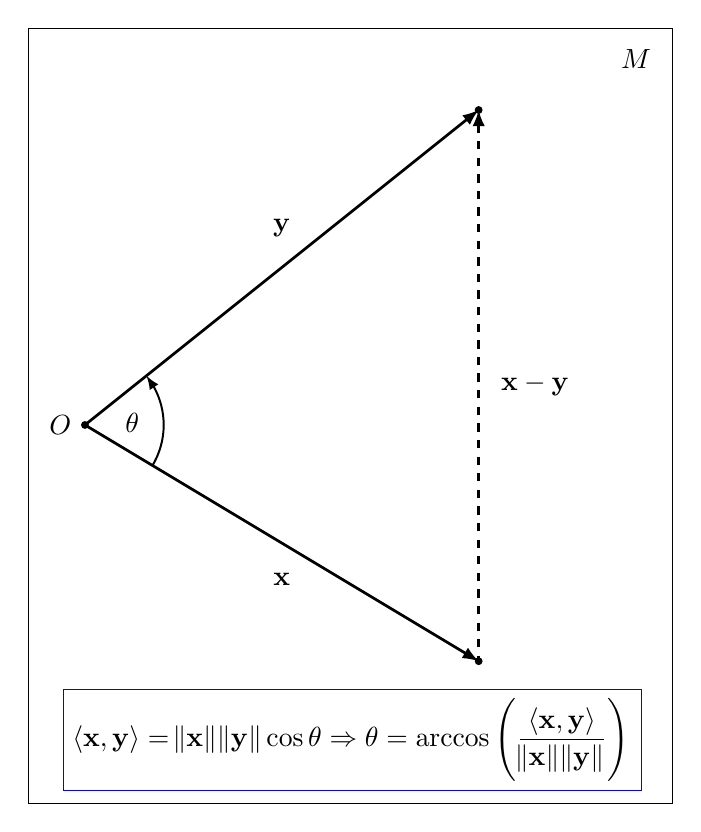
\begin{tikzpicture} [scale=1,framed]							% add a tikz frame
       \coordinate (O)                  at (0,0);               % origin O
       \coordinate (Box)                at (0,-4);				% put the box here (roughtly)
       \coordinate (Xstart)             at (-1,0);              % x-axis 
       \coordinate (Xend)               at (10,0);              % x-axis
       \coordinate (Ystart)             at (0,-1);              % y-axis
       \coordinate (Yend)               at (0, 7.5);            % y-axis
       \coordinate (T)					at (5,4);				% Top point
       \coordinate (B)					at (5,-3);				% bottom point
       \coordinate (TM)					at (2.5,2.00);			% (x,y_1) coordinate
       \coordinate (BM)					at (2.5,-1.50);			% (x,y_2) coordinate 
       \coordinate (M) 					at (7,4.65);			% draw M in upper right corner (x and y generate a plane M)    
%
%
%	Don't draw coordinate system
%       
%	\draw[ultra thick,-latex](Xstart) -- (Xend) node[right,scale=1.75] {$x$};				% x axis
%	\draw[ultra thick,-latex](Ystart) -- (Yend) node[above,scale=1.75] {$y$};				% y axis
%
%
		\draw [line width=0.35mm,-latex] (O) -- (T) node [midway,above,yshift=0.25cm]  {$\mathbf{y}$};	% draw y (top vector)
		\draw [line width=0.35mm,-latex] (O) -- (B) node [midway,below,yshift=-0.25cm] {$\mathbf{x}$};	% draw x (bottom vector)
		\draw [line width=0.35mm,dashed,latex-] (T) -- (B) node [midway,right,xshift=0.15cm]			% draw x-y
			{$\mathbf{x} - \mathbf{y}$};																% continue drawing x - y
		\fill [black] (T) circle (0.05);																% draw a dot, top of x - y
		\fill [black] (B) circle (0.05);																% draw a dot, bottom of x - y
		\node[] at (M) {$M$};

%
%	Draw the angle, box, etc
%     
		\pic [draw,-latex,line width=0.25mm,angle radius=10mm,angle eccentricity=1.2]		% or \pic [...,"${...}$"] {angle = ...}; 
			{angle = BM--O--TM};															% this draws the angle
		\fill [black] (O) circle (0.05) node[below,left,xshift=-0.05cm] {$O$};				% label the origin
		\node [yshift=0.25mm,xshift=6.0mm] at (O) {$\theta$};								% label theta 		
		\node[xshift=7.075cm,below,left,draw,rectangle,color=blue,thin,scale=1] at (Box)	% get \theta = ... in the right place
			{$\color{black}{\langle \mathbf{x},\mathbf{y} \rangle = 
			\norm{\mathbf{x}}\norm{\mathbf{y}} \cos \theta \Rightarrow 
			\theta = \arccos \Bigg(\dfrac{\langle \mathbf{x},\mathbf{y} \rangle}
			{\norm{\mathbf{x}} \norm{\mathbf{y}}} \Bigg )\hspace{0.10em}}$};

%
%	done
%       
   \end{tikzpicture}
  }  																						% end \resizebox
 \caption{Setup for the geometric interpretation of $\langle \mathbf{x},\mathbf{y} \rangle$}
 \label{fig:geometric_inner_product}
\end{figure}


\bigskip
\noindent
If $\theta \in \{0, \pi \}$ is the angle between $\mathbf{x}$ and $\mathbf{y}$ 
in $M$ then by the Law of Cosines \cite{law_of_cosines} we have
\par}

\medskip
\begin{equation}
{\norm{\mathbf{x} - \mathbf{y}}}^2 = {\norm{\mathbf{x}}}^2 + \; 
{\norm{\mathbf{y}}}^2 - 2 \norm{\mathbf{x}} \norm{\mathbf{y}} 
\cos \theta
\label{eqn:law_of_cosines}
\end{equation}


\noindent
We can also notice that 

\begin{equation*}
\begin{array}{lllll}
{\norm{\mathbf{x} - \mathbf{y}}}^2
&=& \sum\limits_{j = 1}^{n} (x_j - y_j)^2
		&\hspace{2em} \mathrel{\#} \text{${\norm{\mathbf{x}}}^2 = \sum\limits_{j = 
					1}^{n} {x}^{2}_{j}$ (Equation (\ref{eqn:magnitude}))}\\
[12pt]
&=& \sum\limits_{j = 1}^{n} \left ( x_{i}^{2} - 2 x_{j} y _{j} + y_{j}^{2} \right )
		&\hspace{2em} \mathrel{\#} (x_j - y_j)^2 = x_{i}^{2} - 2 x_{j} y _{j} + y_{j}^{2} \\
[12pt]
&=& \sum\limits_{j = 1}^{n} x_j ^2 - 2 \sum\limits_{j = 1}^{n} x_j y_j + \sum\limits_{j = 1}^{n} y_j
		&\hspace{2em} \mathrel{\#} \text{sum is a linear operator \cite{wiki:linear_map}} \\
[12pt]
&=& {\norm{\mathbf{x}}}^2 - 2  \langle \mathbf{x} , \mathbf{y} \rangle + \; {\norm{\mathbf{y}}}^2 
 		&\hspace{2em} \mathrel{\#} \text{${\norm{\mathbf{x}}}^2 = \sum\limits_{j = 1}^{n} {x}^{2}_{j}$ 
					and $\langle \mathbf{x},\mathbf{y} \rangle  = \sum\limits_{j =  1}^{n} x_{j} y_{j}$ 
					(Equations (\ref{eqn:magnitude}) and (\ref{eqn:inner}))} \\
[12pt]
&=& {\norm{\mathbf{x}}}^2 + \; {\norm{\mathbf{y}}}^2 - 2  \langle \mathbf{x} , \mathbf{y} \rangle
 		&\hspace{2em} \mathrel{\#} \text{rearrange: ${\norm{\mathbf{x} - \mathbf{y}}}^2 = 
					{\norm{\mathbf{x}}}^2 + \; {\norm{\mathbf{y}}}^2 - 2  \langle \mathbf{x} , 
					\mathbf{y} \rangle$}
\end{array}
\end{equation*}

\bigskip
\noindent
Setting the right-and side (RHS) of this last expression for 
${\norm{\mathbf{x} - \mathbf{y}}}^2$ equal to the RHS of Equation 
(\ref{eqn:law_of_cosines}) yields


\medskip
\begin{equation*}
{\norm{\mathbf{x}}}^2 + \; {\norm{\mathbf{y}}}^2 - 2 \langle \mathbf{x},\mathbf{y} \rangle
=
{\norm{\mathbf{x}}}^2 + \; {\norm{\mathbf{y}}}^2 - 2 \norm{\mathbf{x}} \norm{\mathbf{y}} \cos \theta
\end{equation*}


\bigskip
\noindent
Subtracting ${\norm{\mathbf{x}}}^2 + \; {\norm{\mathbf{y}}}^2$ from both sides
of this equation and then dividing by $-2$ gives us

\medskip
\begin{equation*}
\langle \mathbf{x}, \mathbf{y} \rangle = 
\norm{\mathbf{x}} \norm{\mathbf{y}} \cos \theta
\end{equation*}
\end{theorem}



\medskip
\noindent
\begin{definition} {\bf Orthogonal Vectors:} $\langle \mathbf{x}, \mathbf{y} \rangle = 0$

\bigskip
\noindent
We say that $\mathbf{x}, \mathbf{y} \in \mathbb{R}^{n}$ are
orthogonal if $\langle \mathbf{x}, \mathbf{y} \rangle = 0$, since

\begin{equation*}
\begin{array}{lllll}
\langle \mathbf{x}, \mathbf{y} \rangle 
&=& \norm{\mathbf{x}} \norm{\mathbf{y}} \cos \theta
		&\hspace{5em} \mathrel{\#} \text{Theorem \ref{theorem:ip}} \\
[5pt]
&\Rightarrow& \langle \mathbf{x}, \mathbf{y} \rangle 
		= \norm{\mathbf{x}} \norm{\mathbf{y}} \cos \frac{\pi}{2}
		&\hspace{5em} \mathrel{\#} \mathbf{x} \perp\mathbf{y} \Rightarrow 
		\theta = \frac{\pi}{2} \\
[5pt]
&\Rightarrow& \langle \mathbf{x}, \mathbf{y} \rangle 
		= \norm{\mathbf{x}} \norm{\mathbf{y}} 0
		&\hspace{5em} \mathrel{\#} \cos \frac{\pi}{2} = 0 \\
[5pt]
&\Rightarrow & \langle \mathbf{x}, \mathbf{y} \rangle  = 0
		&\hspace{5em} \mathrel{\#} \norm{\mathbf{x}} \norm{\mathbf{y}} 0 = 0
\end{array}
\end{equation*}
\end{definition}


\smallskip
\begin{definition} 
{\bf Orthogonal Projection} 

\bigskip
\noindent
Given two linearly independent vectors $\mathbf{a},\mathbf{b} \in
\mathbb{R}^{n}$, we want to find the orthogonal projection of
$\mathbf{a}$ onto the line generated by $\mathbf{b}$. To analyze
this, denote by $M$ the plane generated by $\mathbf{a}$
and $\mathbf{b}$ and consider an orthonormal basis
$\{\mathbf{v}_1,\mathbf{v}_2\}$ of $M$ consisting of
$\mathbf{v}_1 = \frac{\mathbf{b}}{\| \mathbf{b} \|}$
($\mathbf{v}_1 = \mathbf{\hat{b}}$) and a unit vector
$\mathbf{v}_2 \in M$ that is orthogonal to $\mathbf{v}_1$.  
This is depicted in Figure \ref{fig:orthogonal_projection}.



\bigskip
\begin{figure}[H]
\center{\includegraphics[scale=0.45] 
{images/orthogonal_projection.png}}
\caption{Orthogonal Projection}
\label{fig:orthogonal_projection}
\end{figure}



\bigskip
\noindent
Since $\{ \mathbf{v}_1, \mathbf{v}_2\}$ is a basis of $M$ there
exist scalars $\alpha$ and $\beta$ such that

\smallskip
\begin{equation}
\mathbf{a} = \alpha \mathbf{v}_1 + \beta \mathbf{v}_2
\label{eqn:alpha_beta}
\end{equation}

\bigskip
\noindent
Here we want to solve for $\alpha$. One way to do that is 
to take the inner product of $\mathbf{b}$ and $\mathbf{a}$ (Equation
(\ref{eqn:alpha_beta})):

\begin{equation*}
\begin{array}{lllll}
\langle \mathbf{a}, \mathbf{b} \rangle
&=& \langle \mathbf{b}, \mathbf{a} \rangle
					&\hspace{3em} \mathrel{\#} \text{since }
					\langle \mathbf{a}, \mathbf{b} \rangle  = 
					\sum\limits_{j = 1}^{n} a_j b_j = 
					\sum\limits_{j = 1}^{n} b_j a_j = 
					\langle \mathbf{b}, \mathbf{a} \rangle
					\text{ (Equation (\ref{eqn:dot_reverse}))} \\
[10pt]
&=& \langle \mathbf{b}, (\alpha \mathbf{v}_1 + \beta \mathbf{v}_2) \rangle
					&\hspace{3em} \mathrel{\#} \text{since } \mathbf{a} = \alpha \mathbf{v}_1 + 
					\beta \mathbf{v}_2 \text{ (Equation (\ref{eqn:alpha_beta}))} \\
[10pt]
&=& \langle \mathbf{b}, \alpha \mathbf{v}_1 \rangle + \langle \mathbf{b}, \beta \mathbf{v}_2 \rangle
					&\hspace{3em} \mathrel{\#} \text{the inner product is distributive 
					over vector addition \cite{wiki:dot_product}} \\
[10pt]
&=& \alpha \langle \mathbf{b},\mathbf{v}_1 \rangle + \beta  \langle \mathbf{b}, \mathbf{v}_2 \rangle
					&\hspace{3em} \mathrel{\#} \text{by the scalar product rule:
					$\! \langle c_{1}\mathbf{v}_1, c_{2}\mathbf{v}_2 \rangle
					= c_{1} c_{2} \langle \mathbf{v}_1, \mathbf{v}_2 \rangle$ \cite{wiki:dot_product}} \\
[10pt]
&=& \alpha \langle \mathbf{v}_{1},\mathbf{b} \rangle + \beta  \langle \mathbf{b}, \mathbf{v}_2 \rangle
					&\hspace{3em} \mathrel{\#} \text{since $\langle \mathbf{b}, \mathbf{v}_1 \rangle 
					= \langle \mathbf{v}_{1},\mathbf{b} \rangle$ (Equation (\ref{eqn:dot_reverse}))} \\
[10pt]
&=& \alpha \langle \mathbf{v}_1, \mathbf{b}\rangle + \beta \, 0
					&\hspace{3em} \mathrel{\#} \text{since }  \langle \mathbf{v}_1, \mathbf{v}_2 \rangle = 0 
					\text{ and } \mathbf{v}_1 = \mathbf{\hat{b}} 
					\Rightarrow \langle \mathbf{\hat{b}}, \mathbf{v}_2  \rangle
					= \frac{1}{\norm{\mathbf{b}}}  \langle \mathbf{b}, \mathbf{v}_2  \rangle
					= 0 
					\Rightarrow  \langle \mathbf{b}, \mathbf{v}_2  \rangle
					= 0 \\
[10pt]
&=& \alpha \langle \mathbf{v}_1, \mathbf{v_1} \norm{\mathbf{b}} \rangle
					&\hspace{3em} \mathrel{\#} \text{since $\beta \, 0 = 0$ and
					$\mathbf{v}_1 = \frac{\mathbf{b}}{\norm{\mathbf{b}}}$
					so $\mathbf{b} = \mathbf{v_1} \norm{\mathbf{b}}$} \\
[10pt]
&=& \alpha \norm{\mathbf{b}} \langle \mathbf{v}_1, \mathbf{v}_1 \rangle
					&\hspace{3em} \mathrel{\#} \text{by the scalar product rule} \\
[10pt]
&=& \alpha \norm{\mathbf{b}}
					&\hspace{3em} \mathrel{\#} \text{since 
					$\mathbf{v}_1 = \frac{\mathbf{b}}{\norm{\mathbf{b}}}
					\Rightarrow \norm{\mathbf{v}_1} = 1
					\text{ and so } \langle \mathbf{v}_1, \mathbf{v_1} \rangle 
					= {\norm{\mathbf{v}_1}}^2 = 1^2 = 1$}
\end{array}
\end{equation*} 


\bigskip
\noindent
So we see that

\medskip
\begin{equation*}
\langle \mathbf{a}, \mathbf{b} \rangle = \alpha \norm{\mathbf{b}}
\end{equation*}

\medskip
\noindent
and so


\begin{equation*}
\alpha
= \dfrac{\langle \mathbf{a}, \mathbf{b} \rangle}{\norm{\mathbf{b}}} 
= \left \langle \mathbf{a}, \dfrac{\mathbf{b}}{\norm{\mathbf{b}}} 
\right \rangle = \langle \mathbf{a}, \mathbf{\hat{b}} \rangle 
\end{equation*}



\bigskip
\noindent
$\alpha$ represents the component of the vector $\mathbf{a}$ that is
parallel to ("in the direction of") the vector $\mathbf{\hat{b}}$. 
More generally, since $\mathbf{\hat{b}}$ is the unit vector in 
the $\mathbf{b}$ direction, 
$\langle \mathbf{a}, \mathbf{b} \rangle$ is also the component 
of $\mathbf{a}$ in the $\mathbf{b}$ direction.
\end{definition}


\bigskip
\begin{definition}
{\bf Cross Product:} $\mathbf{a} \times \mathbf{b}$

\bigskip
\noindent
The cross product is a binary operation on two vectors in a
three-dimensional oriented Euclidean vector space
\cite{euclidian_space}.  Specifically, given two linearly
independent vectors $\mathbf{a}$ and $\mathbf{b}$, the cross
product of $\mathbf{a}$ and $\mathbf{b}$, denoted $\mathbf{a}
\times \mathbf{b}$, is defined to be a vector with the following
three properties:

\bigskip
\begin{itemize}
\item $\mathbf{a} \times \mathbf{b}$ is perpendicular to both
$\mathbf{a}$ and $\mathbf{b}$ (Figure \ref{fig:cross_product_parallelogram}).


\item $\mathbf{a} \times \mathbf{b}$ has direction given by the
right-hand rule (Figure \ref{fig:right_hand_rule_for_cross_products}).

 
\item $\mathbf{a} \times \mathbf{b}$ has magnitude equal to
the area of the parallelogram spanned by $\mathbf{a}$ and
$\mathbf{b}$ (Figure \ref{fig:cross_product_parallelogram}).
\end{itemize}

\bigskip
\begin{figure}[H]
\center{\includegraphics[scale=0.105]
{images/cross_product_parallelogram.png}}
\caption{The parallelogram formed by $\mathbf{a} \times
\mathbf{b}$ \cite{wiki:cross_product}}
\label{fig:cross_product_parallelogram}
\end{figure}


\bigskip
\noindent
One definition of the cross product is 

\bigskip
\begin{equation}
\mathbf{a} \times \mathbf{b} = \norm{\mathbf{a}}
\norm{\mathbf{b}} \sin (\theta) \, \mathbf{n}
\label{eqn:cross_product}
\end{equation}

\bigskip
\noindent
where

\bigskip
\begin{itemize}
\item $\theta$ is the angle between $\mathbf{a}$ and $\mathbf{b}$
in the plane containing them, so $0 \leq \theta \leq \pi$.

\item $\norm{\mathbf{a}}$ and $\norm{\mathbf{b}}$ are the magnitudes 
of the vectors $\mathbf{a}$ and $\mathbf{b}$ (aka their norms; see 
Definition \ref{def:euclidean_norm})). 

\item $\mathbf{n}$ is a unit vector normal to the plane
containing $\mathbf{a}$ and $\mathbf{b}$ in the direction given
by the right-hand rule.
\end{itemize}

\bigskip
\begin{figure}[H]
\center{\includegraphics[scale=0.15] {images/right_hand_rule_cross_product.png}}
\caption{The right-hand rule for vectors $\mathbf{a}$ and 
         $\mathbf{b}$ \cite{wiki:right_hand_rule_for_cross_products}}
\label{fig:right_hand_rule_for_cross_products}
\end{figure}


\medskip
\bigskip
\noindent
If the cross product of two vectors is the zero vector (that is,
$\mathbf{a \times b} = \mathbf{0}$), then either one or both of
the inputs is the zero vector ($\mathbf{a} = \mathbf{0}$ and/or
$\mathbf{b} = \mathbf{0}$) or the vectors are parallel or
anti-parallel ($\theta \in \{0, \pi\}$).  In the second case
($\theta \in \{0, \pi\}$), since the angle between a vector and
itself is zero, Equation (\ref{eqn:cross_product}) tells us that
the cross product of a vector with itself is the zero vector:
$\mathbf{a} \times \mathbf{a} = \norm{\mathbf{a}} 
\norm{\mathbf{a}}  \sin (0) \, \mathbf{n} = \norm{\mathbf{a}} 
 \norm{\mathbf{a}} 0 \, \mathbf{n} = \mathbf{0}$.



\bigskip
\noindent
Note that by the right-hand rule, if the thumb
points at you then the fingers curl in the
anti-clockwise (counter-clockwise) direction. 
That is, when viewed from the top or z 
axis the system rotates in an anti-clockwise
direction. This is one of the reasons we take 
the direction of a curve to be in the anti-clockwise 
direction when we consider, for example, line integrals
in Section \ref{sec:line_integrals}.



\bigskip
\noindent
The cross product can also be expressed as the following
determinant


\bigskip
\begin{equation*}
\mathbf {a\times b} 
= \det \begin{bmatrix}
    \mathbf{\hat{i}} & \mathbf{\hat{j}} & \mathbf{\hat{k}} \\
    a_{1} & a_{2} &a_{3} \\
    b_{1} & b_{2} &b_{3}
  \end{bmatrix} \\
\end{equation*}

\bigskip
\noindent
which can be computed using Sarrus's rule
\cite{wiki:rule_of_sarrus} or cofactor expansion
\cite{cofactor_expansion}. Using Sarrus's rule the cross product
expands to

\bigskip
\begin{equation*}
\begin{aligned}
\mathbf{a\times b} 
&= (a_{2} b_{3} \mathbf{\hat{i}} + a_{3}b_{1} \mathbf{\hat{j}} + a_{1}b_{2} \mathbf{\hat{k}})
-  (a_{3}b_{2}\mathbf{\hat{i}} + a_{1}b_{3}\mathbf{\hat{j}} + a_{2}b_{1}\mathbf{\hat{k}}) \\
&= (a_{2}b_{3} - a_{3}b_{2}) \mathbf{\hat{i}} + ( a_{3}b_{1} - a_{1}b_{3})
\mathbf{\hat{j}} + ( a_{1}b_{2} - a_{2}b_{1} ) \mathbf{\hat{k}} 
\end{aligned}
\end{equation*}

\bigskip
\noindent
Using cofactor expansion the $3 \times 3$ determinant can be 
expressed in terms of $2 \times 2$ determinants:

\bigskip
\begin{equation*}
\begin{aligned}
\mathbf {a\times b} 
&= {\begin{vmatrix}
     a_{2} & a_{3} \\
     b_{2} & b_{3}
    \end{vmatrix}}
    \mathbf{\hat{i}} - 
    {\begin{vmatrix}
      a_{1} & a_{3} \\
      b_{1} & b_{3}
     \end{vmatrix}}
    \mathbf{\hat{j}} +
    {\begin{vmatrix}
      a_{1} & a_{2} \\
      b_{1} & b_{2}
     \end{vmatrix}}
     \mathbf{\hat{k}} \\
&= (a_{2}b_{3} - a_{3}b_{2}) \mathbf{\hat{i}} - 
   (a_{1}b_{3} - a_{3}b_{1}) \mathbf{\hat{j}} +
   (a_{1}b_{2} - a_{2}b_{1}) \mathbf{\hat{k}}
\end{aligned}
\end{equation*}


\bigskip
\noindent
The cross product has the following additional properties \cite{wiki:cross_product}:


\begin{itemize}
\item It is anti-commutative: $\mathbf{a} \times \mathbf{b} 
= - (\mathbf{b} \times \mathbf{a})$


\item It is distributive over addition: $\mathbf{a} \times
(\mathbf{b} + \mathbf{c}) = (\mathbf{a} \times \mathbf{b}) +
(\mathbf{a} \times \mathbf{c})$


\item It is compatible with scalar multiplication so that:
$(c\,\mathbf{a}) \times \mathbf{b} = \mathbf{a} \times
(c\,\mathbf{b}) = c \, (\mathbf{a} \times \mathbf{b})$


\item It is not associative but satisfies the Jacobi identity
\cite{wiki:jacobi_identity}: 
$\mathbf{a} \times (\mathbf{b} \times \mathbf{c}) + 
\mathbf{b} \times (\mathbf{c} \times \mathbf{a}) + 
\mathbf{c} \times (\mathbf{a} \times \mathbf{b}) 
= \mathbf{0}$
\end{itemize}
\end{definition}

\medskip
\section{A Few Theorems}
\bigskip
\begin{theorem} {\bf Cauchy–Schwarz Inequality:} 
$\big | \langle \mathbf{a},\mathbf{b} \rangle \big | \leq 
\norm{\mathbf{a}} \norm{\mathbf{b}}$


\bigskip
{\setstretch {1.50}
\noindent
{\bf Proof.} The inequality is trivial if either $ \mathbf{a}$ or
$\mathbf{b}$ is zero, so assume that neither is. So without loss
of generality (I think) let ${\displaystyle \mathbf{x} =
\frac{\mathbf{a}}{\norm{\mathbf{a}}}}$ and ${\displaystyle
\mathbf{y} = \frac{\mathbf{b}}{\norm{\mathbf{b}}}}$ and so $\norm{
\mathbf{x}} = \norm{\mathbf{y}} = 1$ ($\mathbf{x} =
\mathbf{\hat{a}}$ and $\mathbf{y} = \mathbf{\hat{b}}$).  Then
\par}


\medskip
\begin{equation*}
\begin{array}{lllll}
0
&\leq& \norm{\mathbf{x} - \mathbf{y}}
					&\mathrel{\#} \text{$\norm{\mathbf{x} - \mathbf{y}} \geq 0$ for all 
					$\mathbf{x}, \mathbf{y} \in \mathbb{R}^{n}$ (Equation (\ref{eqn:magnitude}))}\\
[8pt]
&\leq&  {\norm{\mathbf{x} - \mathbf{y}}}^2
					&\mathrel{\#} \norm{\mathbf{x} - \mathbf{y}} \geq 0 
					\Rightarrow  {\norm{\mathbf{x} - \mathbf{y}}}^2 \geq 0 \\ 
[6pt]
&\leq& {\displaystyle \sum\limits_{j = 1}^{n} (x_j - y_j)^2}
					&\mathrel{\#} \text{${\norm{\mathbf{x} - \mathbf{y}}}^2 = {\displaystyle 
					\sum\limits_{j = 1}^{n} {(x_j - y_j)}^2}$ (Equation (\ref{eqn:magnitude}))} \\
[8pt]
&\leq& {\displaystyle \sum\limits_{j = 1}^{n} \left ( x_{j}^2 - 2 x_{j} y_{j} + y_{j}^{2} \right )}
					&\mathrel{\#} \text{expand previous line} \\
[8pt]
&\leq& {\displaystyle \sum\limits_{j = 1}^{n} x_{j}^2 - 2 \sum\limits_{j = 1}^{n} x_{j} y_{j}} 
					+ \sum\limits_{j = 1}^{n} y_{j}^{2}
					&\mathrel{\#} \text{sum is a linear operator} \\
[12pt]
&\leq& {\norm{\mathbf{x}}}^2 - 2 \langle \mathbf{x},\mathbf{y} \rangle + \; {\norm{\mathbf{y}}}^2
					&\mathrel{\#} \text{${\norm{\mathbf{x}}}^2 = \sum\limits_{j = 1}^{n} x_{j}^2$  
					and $\langle \mathbf{x},\mathbf{y} \rangle  = \sum\limits_{j = 1}^{n} x_{j} y_{j}$ 
					(Equations  (\ref{eqn:magnitude}) and (\ref{eqn:inner}) respectively)} \\
[12pt]
&\leq& 1 - 2 \langle \mathbf{x},\mathbf{y} \rangle + 1
					&\mathrel{\#} \norm{\mathbf{x}} = \norm{\mathbf{y}} 
					= 1 \Rightarrow {\norm{\mathbf{x}}}^2 = {\norm{\mathbf{y}}}^2 = 1 \\
[8pt]
&\leq& 2- 2 \langle \mathbf{x},\mathbf{y} \rangle
					&\mathrel{\#} 1 + 1 = 2 \\
[8pt]
&\Rightarrow& -2 \leq -2 \langle \mathbf{x},\mathbf{y} \rangle
					&\mathrel{\#} \text{subtract 2 from both sides}  \\
[8pt]
&\Rightarrow& 1 \geq \langle \mathbf{x},\mathbf{y} \rangle 
					&\mathrel{\#} \text{divide by -2, reversing inequality}  \\
[8pt]
&\Rightarrow& \langle \mathbf{x},\mathbf{y} \rangle \leq 1
					&\mathrel{\#} \text{rearrange}  \\
[4pt]
&\Rightarrow& \left \langle \dfrac{\mathbf{a}}{\norm{\mathbf{a}}}, 
					{\dfrac{\mathbf{b}}{\norm{\mathbf{b}}}} \right\rangle \leq 1
					&\mathrel{\#} \text{$\mathbf{x} 
					= \dfrac{\mathbf{a}}{\norm{\mathbf{a}}}, \; \mathbf{y} 
					= \dfrac{\mathbf{b}}{\norm{\mathbf{b}}}$ by the definition above} \\
[12pt]
&\Rightarrow& \dfrac{\langle \mathbf{a},\mathbf{b} \rangle}{\norm{\mathbf{a}} \norm{\mathbf{b}}} \leq 1
					&\mathrel{\#} \text{scalar multiplication rule:
					$\! \langle c_{1}\mathbf{v}_1, c_{2}\mathbf{v}_2 \rangle 
					= c_{1} c_{2} \langle \mathbf{v}_1, \mathbf{v}_2 \rangle$} \\
[12pt]
&\Rightarrow& \langle \mathbf{a},\mathbf{b} \rangle \leq \norm{\mathbf{a}}\norm{\mathbf{b}}
					&\mathrel{\#} \text{multiply both sides by 
					$\norm{\mathbf{a}} \norm{\mathbf{b}}$}

\end{array}
\end{equation*}

\bigskip
\noindent
If we replace $\mathbf{a}$ by $-\mathbf{a}$ we see by Equation
(\ref{eqn:magnitude}) that $\norm{-\mathbf{a}} = \norm{\mathbf{a}}$. 
Further, by the scalar multiplication rule for inner
products with $c_1 = -1$ and $c_2 = 1$ we have $\langle
-\mathbf{a},\mathbf{b} \rangle = - \langle \mathbf{a},\mathbf{b}
\rangle$. Taken together these results imply that $- \langle
\mathbf{a},\mathbf{b} \rangle \leq \norm{\mathbf{a}} 
\norm{\mathbf{b}}$.


\bigskip
\noindent
Next note that the absolute value of $x$, $|x|$,
is defined to be

\bigskip
\begin{equation}
|x| = {
  \begin{cases}\hfill x, & {\text{if }} x \geq 0 \\
                     -x, & {\text{if }} x < 0.
  \end{cases}
}
\label{eqn:absolute_value}
\end{equation}


\bigskip
{\setstretch{1.30}
\noindent
So one way to see the Cauchy–Schwarz inequality is by setting $x$
equal to $\langle \mathbf{a},\mathbf{b} \rangle$ in Equation
(\ref{eqn:absolute_value}). Then when 
$\langle
\mathbf{a},\mathbf{b} \rangle \geq 0$ we have $\big | \langle
\mathbf{a},\mathbf{b} \rangle \big | = \langle
\mathbf{a},\mathbf{b} 
\rangle$ 
and we showed above that $\langle
\mathbf{a},\mathbf{b} \rangle \leq \norm{\mathbf{a}} \norm{\mathbf{b}}$.  
Similarily, when $\langle \mathbf{a},\mathbf{b} \rangle <
0$ we have $\big | \langle \mathbf{a}, \mathbf{b} \rangle \big |
= - \langle \mathbf{a},\mathbf{b} \rangle$ and we showed that $-
\langle \mathbf{a},\mathbf{b} \rangle \leq \|\mathbf{a}\|
\|\mathbf{b} \|$.  Together these give $\big | \langle
\mathbf{a},\mathbf{b} \rangle \big | \leq \|\mathbf{a}\|
\|\mathbf{b} \|$. Said another way:
$\left [ \left (- \langle \mathbf{a},\mathbf{b} \rangle \leq 
\|\mathbf{a}\| \|\mathbf{b} \| \right ) \land \left ( \langle\mathbf{a},
\mathbf{b} \rangle \leq \|\mathbf{a}\| \|\mathbf{b} \| \right )  \right ]
\Rightarrow \big | \langle \mathbf{a},\mathbf{b} \rangle \big |  
\leq \norm{\mathbf{a}} \norm{\mathbf{b}}$. $\blacksquare$
\par}
\end{theorem}

\section{Derivatives}
We will also denote the derivative of a vector $\mathbf{r}$ with
respect to $t$ by $\dot{\mathbf{r}}$, $\dfrac{d\mathbf{r}}{dt}$
or $\mathbf{r}^{\prime}(t)$.  Note also that by definition

\bigskip
\begin{equation*}
\dfrac{d\mathbf{r}}{dt} := \lim_{\Delta t \to 0}			
			\dfrac{\mathbf{r}(t + \Delta t) - \mathbf{r}(t)}{\Delta t}
\end{equation*}

\section{The Jacobian}
It is common to change the variable(s) of integration with the main
goal being to rewrite a complicated integrand into a some simpler
but equivalent form. However, in doing so, the underlying geometry of
the problem may be altered. This was seen often in
single-variable integrals:

\begin{example} Evaluate 
\begin{equation}
\int_{2}^{4} (3x + 1)^3  dx
\label{eqn:example1}
\end{equation}

\bigskip
\noindent
{\bf Solution}: We can rewrite the integral in Equation
(\ref{eqn:example1}) by letting $u = 3x + 1$ so that $du = 3 \,
dx$. Notice that the expression $du = 3 \, dx \Rightarrow dx =
\frac{1}{3} \, du$ and so the bounds of integration in the
$xy$-plane, namely $2 \leq x \leq 4$ are transformed using $u =
3x + 1$. So if $x = 2$ then $u = 3(2) + 1 = 7$ and when $x = 4$
we have $u = 3(4) + 1 = 13$. So the bounds of integration with
respect to $u$ are $7 \leq u \leq 13$. Using this substitution we
see that

\bigskip
\begin{equation*}
\int_{2}^{4} \! \! (3x + 1)^3 dx 
= \int_{7}^{13} \!\!\!  u^3 \left (\frac{1}{3} \, du \right )
= \frac{1}{3} \int_{7}^{13} \!\!\!  u^3 \, du
\end{equation*}

\bigskip
\setstretch{1.75}
\noindent
Note that integrals ${\displaystyle \int_{2}^{4} (3x + 1)^3 dx}$
and ${\displaystyle \frac{1}{3} \int_{7}^{13} \!\!\!  u^3 \, du}$
represent the same problem. Specifically

\setstretch{1.0}

\bigskip
\begin{equation*}
\int_{2}^{4} \! \! (3x + 1)^3 dx  
=  \left ( \frac{1}{4} \right ) \left ( \frac{1}{3} \right ) \left ( (3x+1)^4 \right ) \Bigg   |_{2}^{4} 
= \left ( \frac{1}{4} \right ) \left ( \frac{1}{3} \right ) \left  ( 13^4 - 7^4 \right ) 
=  \left ( \frac{1}{12} \right ) 26160 
=  2180
\end{equation*}

\bigskip
\noindent
and 

\smallskip
\begin{equation*}
\frac{1}{3} \int_{7}^{13} \!\!\!  u^3 \, du  
=  \left ( \frac{1}{4} \right ) \left ( \frac{1}{3} \right ) \left ( u^4 \right )  \Bigg   |_{7}^{13} 
= \left ( \frac{1}{4} \right ) \left ( \frac{1}{3} \right ) \left (13^4 - 7^4 \right )  
=  \left ( \frac{1}{12} \right ) 26160 
= 2180
\end{equation*}

\bigskip
\noindent
The $\frac{1}{3}$  that we see in the expression 
for $dx$, namely $dx = \frac{1}{3} \, du$ is called the 
(one dimensional) \emph{Jacobian}. 


\bigskip
\noindent
Note also that the integral in variable $x$ is over an interval
of length 2 units, while the integral in $u$ is over an interval
of length 6 units. In a very rough sense then the variable $u$
covers its interval of integration three times “as fast” as
$x$. In particular, since $u$ and $x$ are linearly related the
leading $\frac{1}{3}$ adjusts for the change in the underlying
geometry of the intervals.
\end{example}

\bigskip
\noindent
For double integrals in $\mathbb{R}^2$ we assume that a region of
integration defined in terms of variables $x$ and $y$ and are
substituted for new variables $u$ and $v$ through two functions:

\medskip
\begin{equation*}
\begin{array}{llll}
u = f_1(x,y) \\
[5pt]
v = f_2(x,y)
\end{array}
\end{equation*}

\bigskip
\noindent 
Note that the pair of equations are written so that $u$ and $v$
are written in terms of $x$ and $y$.  This is called a
\emph{transformation}. Such a “change of variables” should also
be reversible.  That is, we should be able to solve for $x$ and
$y$ in terms of $u$ and $v$:

\medskip
\begin{equation*}
\begin{array}{llll}
x = g_1(u,v)  \\
[5pt]
y = g_2(u,v)
\end{array}
\end{equation*}

\bigskip
\noindent
In this case the Jacobian, $J(u,v)$, is defined to be the
determinant of a $2 \times 2$ matrix as follows:

\bigskip
\begin{equation*}
J(u,v)
= \det
\begin{bmatrix}
  \dfrac{\partial g_1}{\partial u} & \dfrac{\partial g_1}{\partial v} \\[2ex]
  \dfrac{\partial g_2}{\partial u} & \dfrac{\partial g_2}{\partial v} 
\end{bmatrix}
= \det
\begin{bmatrix}
  \dfrac{\partial x}{\partial u} & \dfrac{\partial x}{\partial v} \\[2ex]
  \dfrac{\partial y}{\partial u} & \dfrac{\partial y}{\partial v} 
\end{bmatrix}
\end{equation*}

\bigskip
\noindent
In three dimensions the Jacobian is

\bigskip
\begin{equation*}
J(u,v,w) = \det
\begin{bmatrix}
  \dfrac{\partial u}{\partial x}  & \dfrac{\partial u}{\partial y} & \dfrac{\partial u}{\partial z} \\[2ex] 
  \dfrac{\partial v}{\partial x}  & \dfrac{\partial v}{\partial y} & \dfrac{\partial v}{\partial z} \\[2ex]
  \dfrac{\partial w}{\partial x} & \dfrac{\partial w}{\partial y} & \dfrac{\partial w}{\partial z}
\end{bmatrix}
\end{equation*}

\bigskip
\noindent
In general suppose $f: \mathbb{R}^{n} \to \mathbb{R}^{m}$ is a
function such that each of its first-order partial derivatives
exist on $\mathbb{R}^{n}$ This function takes a point $\mathbf{x}
\in \mathbb{R}^{n}$ as input and produces the vector $f(x) \in
\mathbb{R}^{m}$ as output. Then the Jacobian matrix of $f$ is
defined to be an $m \times n$ matrix $J$ whose $(i,j)^\text{th}$
entry is

\begin{equation*}
\mathbf{J}_{ij} = \frac {\partial f_{i}}{\partial x_{j}}
\end{equation*}

\noindent
More explicitly

\begin{equation*}
{\displaystyle \mathbf {J} 
={\det \begin{bmatrix}
 {\dfrac {\partial \mathbf {f} }{\partial x_{1}}} &\cdots & {\dfrac {\partial \mathbf {f} }{\partial x_{n}}}
 \end{bmatrix}}
={\det \begin{bmatrix}
   \nabla ^{\mathrm {T} }f_{1}\\\vdots \\\nabla ^{\mathrm {T} }f_{m}
   \end{bmatrix}}
={\det \begin{bmatrix}
 {\dfrac {\partial f_{1}}{\partial x_{1}}} & \cdots & {\dfrac {\partial f_{1}}{\partial x_{n}}}\\
 \vdots &\ddots &\vdots \\
 {\dfrac {\partial f_{m}}{\partial x_{1}}} & \cdots & {\dfrac {\partial f_{m}}{\partial x_{n}}}
 \end{bmatrix}}}
\end{equation*}

\bigskip
\noindent
where $\nabla^{\mathrm {T} }f_{i}$ is the transpose (row vector)
of the gradient of the $i^{\text{th}}$ component. 


\setstretch{2.0}
\noindent
I have also seen the Jacobian matrix, whose entries are functions
of $\mathbf{x} = [x_1,x_2,\hdots, x_n]$, denoted in various other
ways including ${\displaystyle \nabla \mathbf {f}}$ and
${\displaystyle {\frac {\partial (f_{1},..,f_{m})}{\partial
(x_{1},..,x_{n})}}}$.

\setstretch{1.0}

\begin{figure}[t]
\center{\includegraphics[scale=0.95] {images/r_theta_to_x_y.jpg}}
\caption{Transforming the $r\theta$-plane into the $xy$-plane}
\label{fig:r_theta_to_x_y}
\end{figure}

\medskip
\begin{example} Find the Jacobian for the transformation
shown in Figure \ref{fig:r_theta_to_x_y}.

\bigskip
\noindent
{\bf Solution}: Here we have

\bigskip
\begin{equation*}
\begin{array}{llll}
J(r,\theta)
&=& \det
\begin{bmatrix}
  \dfrac{\partial x}{\partial r} & \dfrac{\partial x}{\partial \theta} \\[2ex]
  \dfrac{\partial y}{\partial r} & \dfrac{\partial y}{\partial \theta} 
\end{bmatrix} 
			&\qquad \qquad \mathrel{\#} \text{definition of the Jacobian} \\
[25pt]
&=& \det
\begin{bmatrix}
  \cos \theta & - r \sin \theta \\
  \sin \theta  & r \cos \theta
\end{bmatrix}
			&\qquad \qquad \mathrel{\#} x = r \cos \theta, y = r \sin \theta \\
[10pt]
&=& \cos (\theta) r \cos (\theta) - (-r \sin (\theta)) \sin (\theta) 
			&\qquad \qquad \mathrel{\#} \det \begin{bmatrix} a & b \\ c & d \end{bmatrix} = ad -bc \\
[10pt]
&=& r \cos^2 \theta + r \sin^2  \theta 
			&\qquad \qquad \mathrel{\#} \text{simplify} \\
[10pt]
&=& r (\cos^2 \theta +  \sin^2 \theta)
			&\qquad \qquad \mathrel{\#} \text{factor out $r$} \\
[10pt]
&=& r
			&\qquad \qquad \mathrel{\#} \cos^2 \theta + \sin^2 \theta = 1
\end{array}
\end{equation*}

\bigskip
\noindent
$J(r,\theta) = r$ is the common Jacobian when rectangular coordinates 
$x$ and $y$ are rewritten in polar coordinates $r$ and $\theta$.
\end{example}

\bigskip
\noindent
For the next example we need the definition of
Type I and Type II regions.

\bigskip
\begin{definition}
{\bf Type I and Type II Regions}

\bigskip
\noindent
A region $D$ in the xy-plane is of Type I if it lies between two
vertical lines and the graphs of two continuous functions
$g_1(x)$ and $g_2(x)$. That is:
$D = \{(x, y) \, | \, a \leq x \leq b, \, g_1(x)  \leq y \leq  g_2(x)\}$.

\bigskip
\noindent
Type I regions are shown in Figure \ref{fig:type_I_region}.


\bigskip
\begin{figure}[H]
\center{\includegraphics[scale=0.35] {images/type_I_region.png}}
\caption{Type I Regions}
\label{fig:type_I_region}
\end{figure}

\bigskip
\noindent
Alternatively, a region $D$ in the xy-plane is of Type II if it
lies between two horizontal lines and the graphs of two
continuous functions $h_1(y)$ and $h_2(y)$. That is

\bigskip
\begin{equation*}
D = \{(x, y) \, | \, c \leq y \leq d, \, h_1(y)  \leq x \leq  h_2(y)\}
\end{equation*}

\bigskip
\noindent
Type II regions are shown in  Figure \ref{fig:type_II_region}.

\bigskip
\begin{figure}[H]
\center{\includegraphics[scale=0.35] {images/type_II_region.png}}
\caption{Type II Regions}
\label{fig:type_II_region}
\end{figure}
\end{definition}


\begin{example}
\setstretch{1.75}
Evaluate ${\displaystyle \iint_{R} (x - 2y) \; dA}$, where $R$ 
is a parallelogram in the $xy$-plane with vertices (0,0), (4,1), 
(6,4) and (2,3). This parallelogram is shown in 
Figure \ref{fig:parallelogram_R}.

\setstretch{1.0}

\medskip
%
%	draw parallelogram for example
%
\begin{figure}[H]
\centering
  \resizebox{0.50 \textwidth}{!} {																% resize figure if you want
  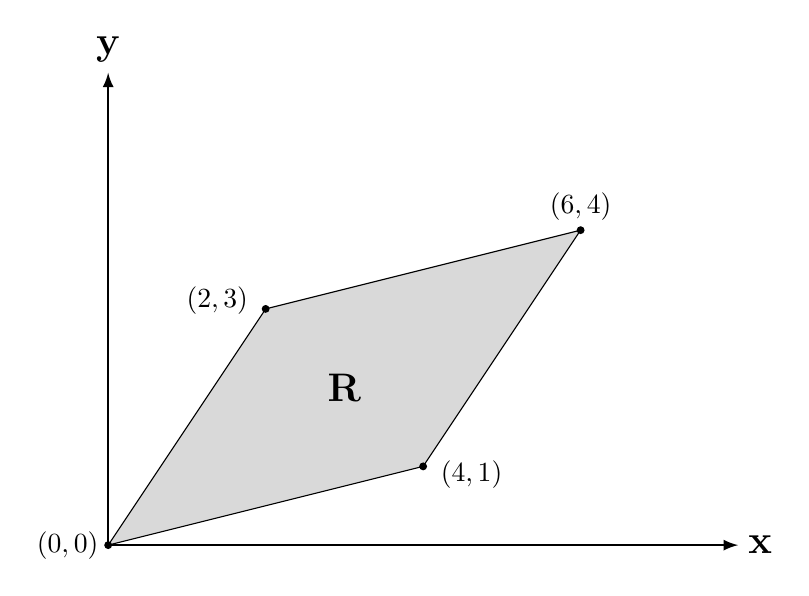
\begin{tikzpicture}
       \coordinate (O)		at (0,0);															% origin O
       \coordinate(Xend)	at (8,0);															% x-axis out to 8
       \coordinate(Yend)	at (0,6);															% y-axis up to 6
       \coordinate(C1)		at (2,3);															% parallelogram point
       \coordinate(C2)		at (6,4);															% parallelogram point
       \coordinate(C3)		at (4,1); 															% parallelogram point
       \coordinate(C)		at (3,2);															% center of parallelogram is at C
%
%	draw axes
%
     \draw[thick,-latex] (O) -- (Xend) coordinate [label={[right] {\Large ${\mathbf{x}}$}}];	% x axis
     \draw[thick,-latex] (O) -- (Yend) coordinate [label={[above] {\Large ${\mathbf{y}}$}}];	% y axis
%
%	draw parallelogram
%
     \draw [fill=gray!30]  (O) -- (C1) -- (C2) -- (C3) -- cycle;
     \node[color=black,font=\Large] at (C) {$\mathbf{R}$};
     \fill [black] (O)   circle (0.05)  node[below,left]{$(0,0)$};
     \fill [black] (C1) circle (0.05)  node[yshift=1.0mm, xshift=-1.0mm, left] {$(2,3)$};
     \fill [black] (C2) circle (0.05)  node[above] {$(6,4)$};
     \fill [black] (C3) circle (0.05)  node[yshift=-1.00mm, xshift=1.0mm,right] {$(4,1)$};
  \end{tikzpicture}
  }	
  \caption{Parallelogram in the $xy$-plane}
  \label{fig:parallelogram_R}
\end{figure}

% \bigskip
% \begin{figure}[H]
% \center{\includegraphics[cfbox=black,scale=0.65] {images/parallelogram_R.png}}
% \caption{Parallelogram in the xy-plane}
% \label{fig:parallelogram_R}
% \end{figure}

\bigskip
\noindent
{\bf Solution}: A sketch of this region (Figure
\ref{fig:parallelogram_R}) shows that it is a Type II region and
would require three separate double integrals in either the $dy$,
$dx$ or $dx dy$ orderings of integration.  Instead, note that the
region consists of two pairs of parallel sides and so we can find
the equation for each side:


\bigskip
\begin{itemize}
\item For the region from $(0,0)$ to $(4,1)$ we have $y = \frac{1}{4}x$ or $-x + 4y = 0$
\item For the region from $(2,3)$ to $(6,4)$ we have $y = \frac{1}{4}x + \frac{5}{2}$ or $-x + 4y = 10$
\item For the region from $(0,0)$ to $(2,3)$ we have $y = \frac{3}{2}x$ or $-\frac{3}{2}x$  or  $-3x + 2y = 0$
\item For the region from $(4,1)$ to $(6,4)$ we have $y = \frac{3}{2}x - 5$ or $-3x + 2y = -10$
\end{itemize}

\bigskip
\noindent
This is shown in Figure \ref{fig:parallelogram_sides}.

\bigskip
%
%	draw parallelogram for example
%
\begin{figure}[H]
\centering
  \resizebox{0.75 \textwidth}{!} {                      % resize figure if you want
  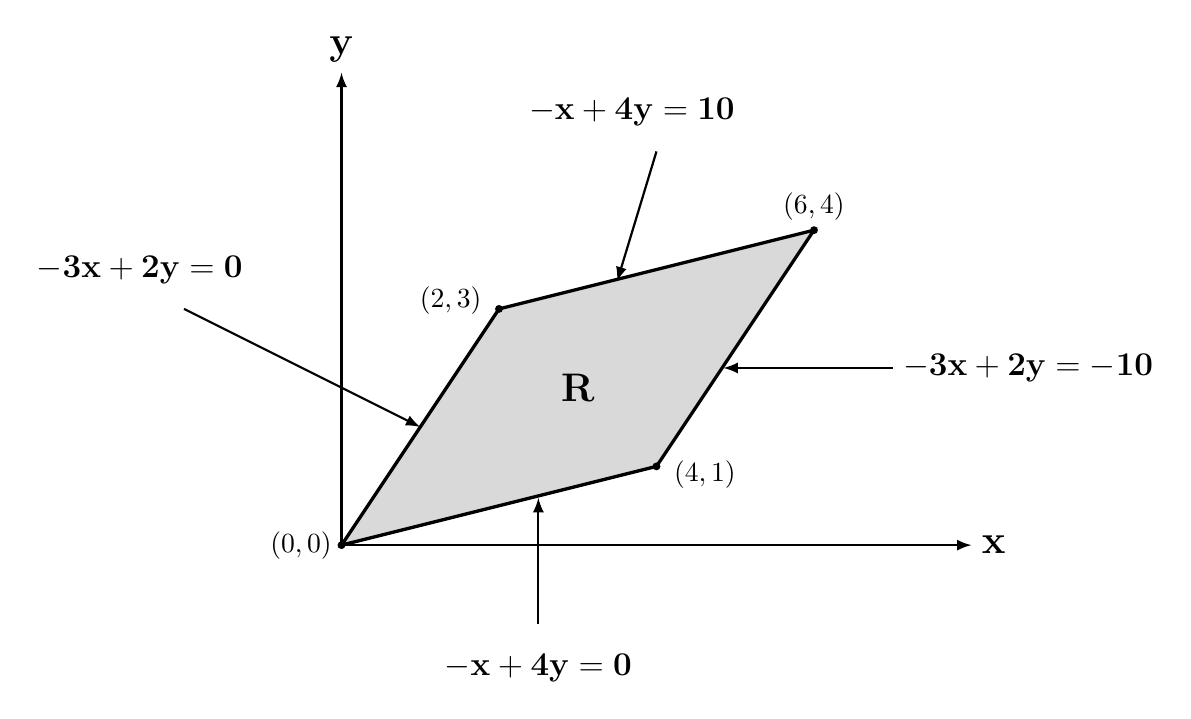
\begin{tikzpicture}
       \coordinate (O)          at (0,0);               % origin O
       \coordinate (Xend)       at (8,0);               % x-axis out to 8
       \coordinate (Yend)       at (0,6);               % y-axis up to 6
       \coordinate (C1)         at (2,3);               % parallelogram point
       \coordinate (C2)         at (6,4);               % parallelogram point
       \coordinate (C3)         at (4,1);               % parallelogram point
       \coordinate (C)          at (3,2);               % center of parallelogram is at C
%
%	coordinates for equations
%  
       \coordinate (D1)         at (1.00, 1.50);
       \coordinate (D2)         at (-2.00,3.00);
       \coordinate (E1)         at (3.50, 3.35);
       \coordinate (E2)         at (4.00, 5.00);
       \coordinate (F1)         at (4.85, 2.25);
       \coordinate (F2)         at (7.00, 2.25);
       \coordinate (G1)         at (2.50, 0.60);
       \coordinate (G2)         at (2.50,-1.00);
%
%	draw axes
%
     \draw[thick,-latex] (O) -- (Xend) coordinate [label={[right] {\Large ${\mathbf{x}}$}}];	% x axis
     \draw[thick,-latex] (O) -- (Yend) coordinate [label={[above] {\Large ${\mathbf{y}}$}}];	% y axis
%
%	draw parallelogram
%
     \draw [very thick,fill=gray!30]  (O) -- (C1) -- (C2) -- (C3) -- cycle;
     \node[color=black,font=\Large] at (C) {${\mathbf{R}}$};
     \fill [black] (O)  circle (0.05) node[below,left] {$(0,0)$};
     \fill [black] (C1) circle (0.05) node[left,yshift=1.0mm,xshift=-1.0mm] {$(2,3)$};
     \fill [black] (C2) circle (0.05) node[above] {$(6,4)$};
     \fill [black] (C3) circle (0.05) node[right,yshift=-1.00mm,xshift=1.0mm] {$(4,1)$};
%
%	draw equations of each size
%       
     \draw [thick,latex-] (D1) -- (D2) coordinate [label={[font=\large,right,xshift=-2.0cm,yshift=0.50cm] 
                ${\mathbf {-3x + 2y = 0}}$}];
     \draw [thick,latex-] (E1) -- (E2) coordinate [label={[font=\large,right,xshift=-1.75cm,yshift=0.5cm] 
                ${\mathbf {-x + 4y = 10}}$}];
     \draw [thick,latex-] (F1) -- (F2) coordinate [label={[font=\large,right]
                ${\mathbf {-3x + 2y = -10}}$}];
     \draw [thick,latex-] (G1) -- (G2) coordinate [label={[font=\large,below,yshift=-0.25cm] 
                ${\mathbf {-x + 4y = 0}}$}];
  \end{tikzpicture}
  }	
  \caption{Equations of the sides of the parallelogram shown in Figure \ref{fig:parallelogram_R}}
  \label{fig:parallelogram_sides}
\end{figure}

\bigskip
\noindent
Now we can define a transformation from $x$ and $y$ into the new variables $u$ and $v$
by the following equations:

\bigskip
\begin{equation*}
\begin{array}{lllll}
&u = -x + 4y  &&& \mathrel{\#} \text{so that $0 \leq u \leq 10$} \\
[5pt]
&v = -3x + 2y &&& \mathrel{\#} \text{so that $-10 \leq v \leq 0$}
\end{array}
\end{equation*}

\bigskip
\noindent
This transformation transforms the region of integration 
$\mathbf{R}$ in the $xy$-plane (a parallelogram,
Figure \ref{fig:parallelogram_R}) into a square in the
$uv$-plane and so $u$ and $v$ have constant bounds. This
square is shown Figure \ref{fig:transformation_uv_plane}. 
The double-integral (whether written in $xy$-space or $uv$-space) 
should be negative because the integrand is "more often" 
negative over $\mathbf{R}$ and its transform into
the $uv$-space.

%
%	draw the transformation: square in the uv-plane
%
\begin{figure}[H]
\centering
  \resizebox{0.50 \textwidth}{!} {                      % resize figure if you want
  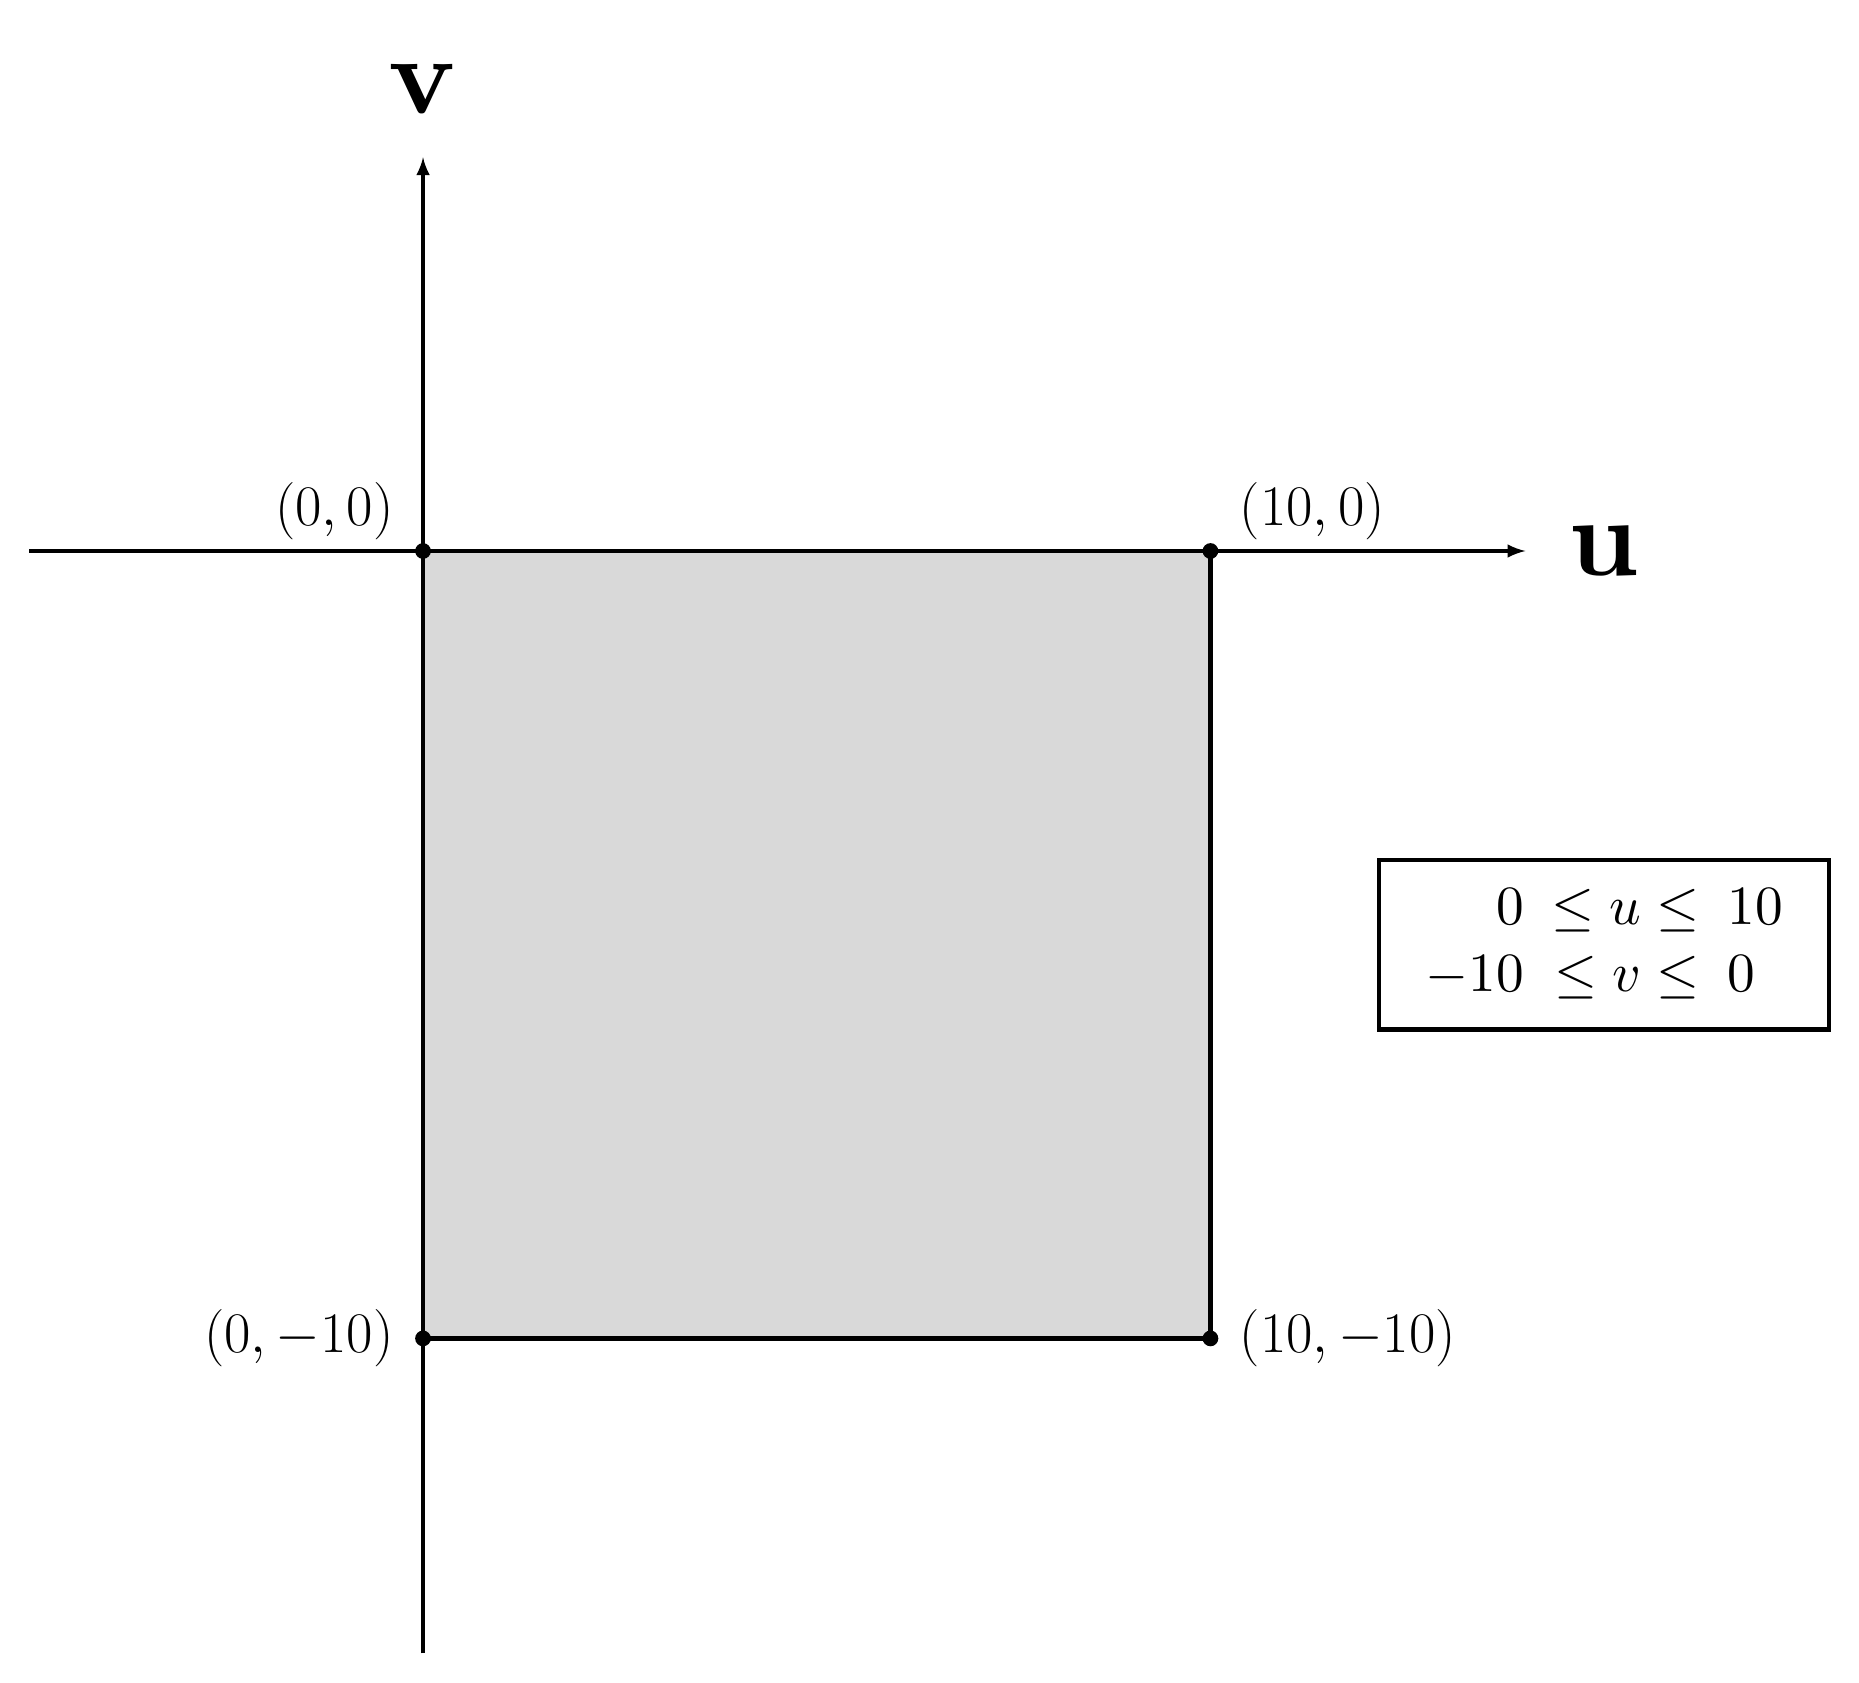
\begin{tikzpicture}
       \coordinate (O)          at (0,0);				% origin O 
       \coordinate (Xstart)     at (-5,0);				% x-axis start
       \coordinate (Xend)       at (14,0);              % x-axis end
       \coordinate (Ystart)     at (0,-14);             % y-axis start
       \coordinate (Yend)       at (0, 5);              % y-axis end
       \coordinate (xy1)        at (0,-10);             % parallelogram point
       \coordinate (xy2)        at (10,-10);            % parallelogram point
       \coordinate (xy3)        at (10,0);				% parallelogram point
       \coordinate (E)          at (15,-5);				% put the box with the bounds here
%
%	draw parallelogram
%
%
       \draw [ultra thick, fill=gray!30] (xy1) -- (O) -- (xy3) -- (xy2) -- cycle;
       \fill [black] (O)   circle (0.10) node[font=\huge,above,left,xshift=-0.25cm,yshift=0.5cm]  {$(0,0)$};
       \fill [black] (xy1) circle (0.10) node[font=\huge,left,xshift=-0.25cm]                     {$(0,-10)$};
       \fill [black] (xy2) circle (0.10) node[font=\huge,right,xshift=0.25cm]                     {$(10,-10)$};
       \fill [black] (xy3) circle (0.10) node[font=\huge,above,right,xshift=0.25cm,yshift=0.50cm] {$(10,0)$};
%     
%	draw axes making sure axes are on top
%
       \draw[very thick,-latex](Xstart) -- (Xend) node[right,scale=4.0] {${\mathbf{u}}$};				% u axis
       \draw[very thick,-latex](Ystart) -- (Yend) node[above,scale=4.0] {${\mathbf{v}}$};				% v axis  
%
%	draw the bounds in a box
%
 	   \node[ultra thick,draw,rectangle,scale=2.0] at (E) {$\begin{array}{rrlrr}
                                                               0 \!\!\! &\leq u \leq& \!\!\! 10 \\
                                                             -10 \!\!\! &\leq v \leq& \!\!\! 0
                                                            \end{array}$};
%
%	done
%       
   \end{tikzpicture}
  }																										% end \resizebox
 \caption{The parallelogram $\mathbf{R}$ (Figure \ref{fig:parallelogram_R}) is a square in the $uv$-plane}
 \label{fig:transformation_uv_plane}
\end{figure}

\bigskip
\noindent
Now we need to solve for $x$ and $y$. We have expressions 
for $u$ and $v$ and so can solve for $x$ and $y$:

\bigskip
\begin{equation*}
\begin{array}{llll}
&u = -x + 4y \\
&v = -3x + 2y 
\end{array}
\end{equation*}

\bigskip
\noindent
First multiply the bottom row by -2:


\bigskip
\begin{equation*}
\begin{array}{rrll}
&u &=& -x + 4y \\
&-2 v &=& -2 (-3x + 2y) 
\end{array}
\end{equation*}

\bigskip
\noindent
Simplifying we get

\bigskip
\begin{equation}
\begin{array}{rrrr}
&u &=& -x + 4y \\
&-2 v &=& 6x - 4y 
\label{eqn:equations_for_u_and_v}
\end{array}
\end{equation}

\bigskip
\noindent
Adding these two equations we get $u - 2v = 5x$
and so solving for $x$ we get

\bigskip
\begin{equation}
x = \frac{1}{5} u - \frac{2}{5} v
\label{eqn:transformation_x}
\end{equation}

\bigskip
\noindent
Substituting this back into the equation for $u$ 
in Equations (\ref{eqn:equations_for_u_and_v})
and solving for $y$ we get

\bigskip
\begin{equation}
y = \frac{3}{10} u - \frac{1}{10} v
\label{eqn:transformation_y}
\end{equation}

\bigskip
\noindent
We can now find the Jacobian:

\begin{equation*}
\begin{array}{lllll}
J(u,v) 
&=& \det
\begin{bmatrix}
  \dfrac{\partial x}{\partial u} & \dfrac{\partial x}{\partial v} \\[2ex]
  \dfrac{\partial y}{\partial u} & \dfrac{\partial y}{\partial v} 
\end{bmatrix} 
			&\qquad \mathrel{\#} \text{definition of the Jacobian} \\
[25pt]
&=& \det
\begin{bmatrix}
  \dfrac{1}{5}  & - \dfrac{2}{5} \\[2ex]
  \dfrac{3}{10} & - \dfrac{1}{10} 
\end{bmatrix} 
			&\qquad \mathrel{\#} x = \frac{1}{5} u - \frac{2}{5} v \text{ and } y = \frac{3}{10} u - \frac{1}{10} v \\
[25pt]
&=& \Bigg [\left(\dfrac{1}{5}\right )\left ( - \dfrac{1}{10}\right ) \Bigg ] 
 -  \Bigg [\left ( - \dfrac{2}{5} \right ) \left (\dfrac{3}{10}\right )  \Bigg ]
			&\qquad \mathrel{\#} \det \begin{bmatrix} a & b \\ c & d \end{bmatrix} = ad -bc \\
[15pt]
&=& - \dfrac{1}{50} + \dfrac{6}{50}
			&\qquad \mathrel{\#} \text{simplify} \\
[10pt]
&=& \dfrac{5}{50}
			&\qquad \mathrel{\#} \text{simplify} \\
[10pt]
&=& \dfrac{1}{10}
			&\qquad \mathrel{\#} J(u,v) = \dfrac{1}{10}

\end{array}
\end{equation*}

\bigskip
\noindent
So we see that the Jacobian in this case is

\begin{equation}
J(u,v) = \dfrac{1}{10}
\label{eqn:jacobian}
\end{equation}

\bigskip
\noindent
Substituting Equations (\ref{eqn:transformation_x}) and 
(\ref{eqn:transformation_y}) into the original  
integral and noting that $dA = J(u,v) \, du \, dv$ we 
get

\begin{equation*}
\begin{array}{lllll}
{\displaystyle \iint\limits_{R} (x - 2y) \, dA}
&=& {\displaystyle \int\limits_{-10}^{0} \int\limits_{0}^{10} \left ( \left (  \dfrac{1}{5}u - \dfrac{2}{5}v \right )
 -  2 \left( \dfrac{3}{10} u  - \dfrac{1}{10} v \right ) \right )}
 \left ( \dfrac{1}{10} \right ) du \, dv
			&\mathrel{\#} \text{\small Equations (\ref{eqn:transformation_x}) \& (\ref{eqn:transformation_y})
			and $dA = \left ( \frac{1}{10} \right ) du \, dv$}

\\
[25pt]
&=& {\displaystyle \dfrac{1}{10} \int\limits_{-10}^{0} \int\limits_{0}^{10}}
    \left ( - \dfrac{2}{5} u - \dfrac{1}{5} v \right ) du \, dv
			&\hspace{-4em} \mathrel{\#} \text{\small simplify, moving the Jacobian to the front} \\
[25pt]
&=& {\displaystyle \dfrac{1}{10} \int\limits_{-10}^{0} \! (-20 -2v) \,dv}
			&\hspace{-4em} \mathrel{\#} {\small {\displaystyle \int\limits_{0}^{10} \! \left ( - \dfrac{2}{5} u - \dfrac{1}{5} v \right ) du}
			= \left [ - \dfrac{1}{5} u^2 - \dfrac{1}{5} uv \right ] \Bigg |_{0}^{10}} \\
[25pt]
&=& \dfrac{1}{10} \Big [ -20 v - v^2 \Big ] \bigg |_{-10}^{0}
			&\hspace{-4em} \mathrel{\#} \text{\small evaluate integral + FToC} \\
[25pt]
&=& 0 - \dfrac{1}{10}  \bigg [ - 20 (-10) - (-10)^2  \bigg ] 
			&\hspace{-4em} \mathrel{\#} \text{\small evaluate at limits} \\
[25pt]
&=& \left (-\dfrac{1}{10} \right ) (100)
			&\hspace{-4em} \mathrel{\#} {\small \bigg ( - \dfrac{1}{10} \bigg ) \big ( 200 - 100 \big ) = -\dfrac{1}{10} (100)}\\
[25pt]
&=& -10
			&\hspace{-4em} \mathrel{\#} \text{\small the region is completely below the $u$ axis} \\
[15pt]
&\Rightarrow& {\displaystyle \Bigg | \iint\limits_{R} (x - 2y) \, dA} \Bigg | = 10
			&\hspace{-4em} \mathrel{\#} \text{\small the volume is $10 \text{ units}^3$} \\

\end{array}
\end{equation*}

 

\bigskip
\noindent
This was an example of a linear transformation, 
in which the equations transforming $x$ and $y$ into $u$ and 
$v$ were \emph{linear} (so were the equations reversing the
transformation). When this is the case the Jacobian will be 
a constant like we saw here.

\bigskip
\setstretch{1.10}
\noindent
We can also see how the geometry changed: The original region in
the $xy$-plane has an area of $10 \text{ units}^2$ while the
region in the $uv$-plane has an area of $100 \text{ units}^2$.
That is, the region in the $uv$-plane is 10 times as large as the
region in the $xy$-plane. The Jacobian $\left (\frac{1}{10}
\right )$ scales this change in the underlying area.

\setstretch{1.0}

\bigskip
\begin{remark}
Note that the Jacobian is usually taken to be a positive
quantity.  This is because the naming (and ordering) of the
functions transforming $x$ and $y$ into $u$ and $v$ (and the
reverse) is arbitrary. Since the Jacobian is a determinant, it is
possible that two rows may be swapped depending on the original
naming of the functions, which may introduce a factor of $-1$
into the result, which can be ignored.
\label{remark:minus_jacobian}
\end{remark}
\end{example}

\section{Arc Length}
\label{sec:arc_length}
Consider a segment of the parametric curve $\mathbf{r}(t) = g(t) \,
\hat{\mathbf{i}} + h(t) \, \hat{\mathbf{j}} + k(t) \,
\hat{\mathbf{k}}$ between two points $P =\mathbf{r}(t)$ and $Q
=\mathbf{r}(t + \Delta t)$, as shown in Figure \ref{fig:delta-r}.

\bigskip
\noindent
A question we might ask is: what is the length of the segment 
of the curve between $P$ and $Q$? This length is called the arc
length and is denoted by $\Delta s$ and can be approximated
by the chord length $\| \Delta \mathbf{r} \|$. 



\bigskip
\begin{figure}[H]
\center{\includegraphics[scale=0.40] {images/delta-r.png}}
\caption{$\Delta \mathbf{r} = \mathbf{r}(t + \Delta t) - \mathbf{r}(t)$}
\label{fig:delta-r}
\end{figure}


\bigskip
\noindent
Specifically we can see from Figure \ref{fig:delta-r} that

\medskip
\begin{equation*}
\| \Delta r \| = \| \mathbf{r}(t + \Delta t) - \mathbf{r}(t) \|	
\end{equation*}

\medskip
\noindent
and so

\begin{equation*}
\Delta s \approx \| \mathbf{r}(t + \Delta t) - \mathbf{r}(t) \|	
\end{equation*}

\bigskip
\noindent
Now we can compute the infinitesimal arc length $ds$,
as shown in Figure \ref{fig:pythagorean_theorem}:

\bigskip
\bigskip
%
%	draw Pythagorean theorem stuff
%
\begin{figure}[H]
\centering
  \resizebox{0.60 \textwidth}{!} {																							% resize figure if you want 
  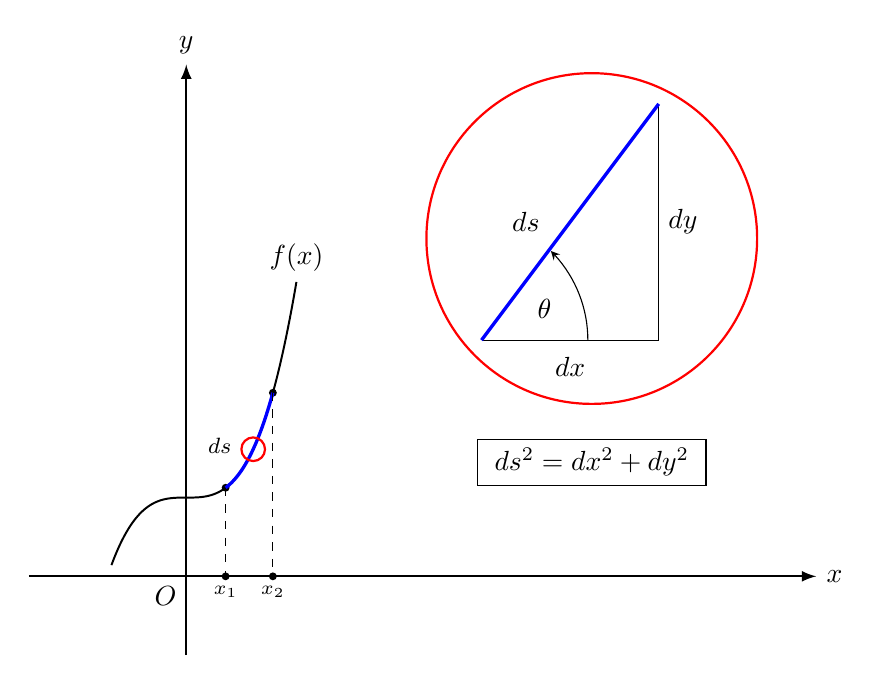
\begin{tikzpicture} [every edge quotes/.append style = {anchor=south, sloped},declare function={f(\x)=1 + \x*\x*\x;}]		% define f(x)
       \draw[thick, -latex] (-2,0) -- (8.0,0.0) coordinate [label={[right] $x$}];  											% x axis
       \draw[thick, -latex] (0,-1) -- (0,6.5) coordinate [label={[above] $y$}]; 											% y axis
       \draw [line width=0.25mm, smooth,samples=100,domain=-0.95:1.40] plot (\x,{f(\x)});									% draw f(x)
       \draw [draw=none] (1.40, {f(1.40)}) coordinate [label={[above] $f(x)$}];												% label f(x)
       \coordinate (O) at (0,0); 																							% origin
       \path (O) node[below left] {$O$};																					% draw origin
%
%	various coordinates
%     
       \coordinate (x1y1) at (0.5,{f(0.5)});
       \coordinate (x1y0) at (0.5,0.0);
       \coordinate (x2y2) at (1.1,{f(1.1});
       \coordinate (x2y0) at (1.1,0.0);
       \coordinate (cir)  at (0.85,{f(0.85)});
%
       \fill (x1y1) circle (0.05);																					% put a dot on the curve at x1y1
       \fill (x2y2) circle (0.05);																					% put a dot on the curve at x2y2
	   \draw [very thick,blue,smooth,samples=100,domain=0.5:1.1] plot (\x,{f(\x)});											% draw blue segment on f(x)
       \draw[draw=none] (x1y1) -- (x2y2) coordinate [label={[font=\footnotesize,yshift=-0.065cm,xshift=-0.105cm,midway,left] \color{black} $ds$}];
       \draw[dashed] (x1y1) -- (x1y0) coordinate [label={[font=\scriptsize,below] \color{black} $x_1$}];
       \draw[dashed] (x2y2) -- (x2y0) coordinate [label={[font=\scriptsize,below] \color{black} $x_2$}];
       \fill (x1y0) circle (0.05);              																			% put a dot on the x axis at x1
       \fill (x2y0) circle (0.05);                      																		% put a dot on the x axis at x2
       \draw[red, thick] (cir) circle (0.150);																				% put a circle on f(x) where ds is
       

     
%
%	draw triangle and circle to show ds
%   
%
%
%	set up triangle coordinates
%
	   \coordinate (a) at (3.75,3.00);
	   \coordinate (c) at (6.00,3.00);
	   \coordinate (b) at (6.00,6.00);
%
%	draw the triangle
%	   
       \draw[] (a) -- (c) coordinate [label={[yshift=-0.1cm,midway,below] ${dx}$}];											% dx
       \draw[] (c) -- (b) coordinate [label={[midway,right] ${dy}$}];														% dy
       \draw[blue,very thick] (a) -- (b) coordinate [label={[xshift=-0.25cm,midway,left] \color{black} ${ds}$}];			% ds
       \draw[red,thick] (5.15,4.29) circle (2.10);																			% big circle
       \draw[draw=none] (0,0) -- (5.15,1.75)  node[draw,rectangle,below] {${\; ds^2 = dx^2 + dy^2 \;}$};					% draw the pythagorean theorem
%
%	draw the angle      
%       
       \node[xshift=-2mm, yshift=-2mm] at (4.75,3.60) {$\theta$};
       \draw[-stealth,thin] (5.10,3.00) arc (0:45:1.60cm);
%
%	done
%
     \end{tikzpicture}
    }																					 									% end resizebox                                                            
 \caption{$f(x)$, $ds$ and the Pythagorean Theorem}
 \label{fig:pythagorean_theorem}
 \end{figure}


\begin{equation*}
\begin{array}{lllll}
\Delta s
&\approx& \| \Delta \mathbf{r} \|							
			&\qquad \mathrel{\#} \text{approximate $\Delta s$ by $\| \Delta \mathbf{r} \|$} \\
[15pt]
&=& \| \mathbf{r}(t + \Delta t) - \mathbf{r}(t) \|		
			&\qquad \mathrel{\#} \Delta \mathbf{r}= \mathbf{r}(t + \Delta t) - \mathbf{r}(t) \\
[15pt]
&=& \| \mathbf{r}(t + \Delta t) - \mathbf{r}(t) \| \cdot \dfrac{\Delta t}{\Delta t} 
			&\qquad \mathrel{\#} \text{multiply by $1 = \dfrac{\Delta t}{\Delta t}$} \\
[15pt]
&=& \bigg \| \dfrac{\mathbf{r}(t + \Delta t) - \mathbf{r}(t)}{\Delta t} \bigg \| \cdot  \Delta t 
			&\qquad \mathrel{\#} \text{assume $\Delta t > 0$} \\
[15pt]
&\Rightarrow& \Delta s \approx \bigg \| \dfrac{\mathbf{r}(t + \Delta t) - 
			\mathbf{r}(t)}{\Delta t} \bigg \| \cdot  \Delta t
			&\qquad \mathrel{\#} \text{combine expressions for $\Delta s$} \\
[15pt]
&\Rightarrow& {\displaystyle \lim_{\Delta t \to 0} \Delta s =  \lim_{\Delta t \to 0} \Bigg [ 			
			\bigg \| \dfrac{\mathbf{r}(t + \Delta t) - \mathbf{r}(t)}{\Delta t} \bigg \| \cdot \Delta t} \Bigg ]
			&\qquad \mathrel{\#} \text{take the limit of both sides} \\
[15pt]
&\Rightarrow& {\displaystyle ds = \lim_{\Delta t \to 0} \Bigg  [ \bigg \| 			
			\dfrac{\mathbf{r}(t + \Delta t) - \mathbf{r}(t)}{\Delta t} \bigg \| \cdot \Delta t} \Bigg ] 
			&\qquad \mathrel{\#} \text{$\Delta t \to 0 \Rightarrow \Delta s \to 0 \Rightarrow \!\!
			{\displaystyle \lim_{\Delta t \to 0} \Delta s = ds}$} \\
[15pt]
&\Rightarrow& {\displaystyle ds = \lim_{\Delta t \to 0} \bigg \| 			
			\dfrac{\mathbf{r}(t + \Delta t) - \mathbf{r}(t)}{\Delta t} \bigg \|
			\cdot \lim_{\Delta t \to 0} \Delta t}
			&\qquad \mathrel{\#} \text{product rule for limits \cite{properties_of_limits}} \\
[15pt]
&\Rightarrow& {\displaystyle ds =  \bigg \| \lim_{\Delta t \to 0}			
			\dfrac{\mathbf{r}(t + \Delta t) - \mathbf{r}(t)}{\Delta t} \bigg \|
			\cdot \lim_{\Delta t \to 0} \Delta t}
			&\qquad \mathrel{\#} \text{for a normed vector space ${\displaystyle X \; \lim \|x_n\| = \|\lim x_n \|}$} \\
[15pt]
&\Rightarrow& ds = \bigg \| \dfrac{d\mathbf{r}}{dt} \bigg \| \cdot dt
			&\qquad \mathrel{\#} {\displaystyle \lim_{\Delta t \to 0}			
			\dfrac{\mathbf{r}(t + \Delta t) - \mathbf{r}(t)}{\Delta t} = \dfrac{d\mathbf{r}}{dt},
			\; \lim_{\Delta t \to 0} \Delta t} = dt
\end{array}
\end{equation*}


\bigskip
\noindent
Interestingly we can also see this using the Pythagorean theorem.
Specifically, if we move an infinitesimal distance in the $x$ and
$y$ directions we get a triangle in the $xy$-plane who's sides
have length $dx$ and $dy$ and who's hypotenuse is $ds$. This
scenario is shown for some curve $f(x)$ in Figure \ref{fig:pythagorean_theorem}. 
In the two dimensional case where the parameterization is $x = g(t)$ 
and $y = h(t)$ we define $\mathbf{r}(t) = g(t) \, \hat{\mathbf{i}} + 
h(t) \, \hat{\mathbf{j}}$ so that

\bigskip
\begin{equation}
\dfrac{d\mathbf{r}}{dt} = \dfrac{dg}{dt} \, \hat{\mathbf{i}} + \dfrac{dh}{dt} \, \hat{\mathbf{j}}
\label{eqn:drdt}
\end{equation}


\bigskip
\noindent
The Pythagorean theorem tells us that 
$ds = \sqrt{dx^2 + dy^2}$. Using
this expression for $ds$ we can see that

\bigskip
\begin{equation*}
\begin{array}{lllll}
ds
&=& \sqrt{dx^2 + dy^2}				
			&\hspace{2em} \mathrel{\#} \text{Figure \ref{fig:pythagorean_theorem}} \\
[14pt]
&=& \sqrt{dg^2 + dh^2}	
			&\hspace{2em} \mathrel{\#} \text{switch to parametric form: 
			$x = g(t)$ and $y = h(t)$} \\
[14pt]
&=& \sqrt{{dg}^2 + {dh}^2} \cdot \dfrac{dt}{dt}
			&\hspace{2em} \mathrel{\#} \text{multiply by 
			$1 = \dfrac{dt}{dt}, \; dt > 0$}  \\
[14pt]
&=& \sqrt{{dg}^2 + {dh}^2} \cdot \Bigg [\sqrt{\dfrac{1}{{dt}^2}} \cdot dt \Bigg ]
			&\hspace{2em} \mathrel{\#} \dfrac{dt}{dt} 
			= \sqrt{\left (\dfrac{dt}{dt} \right)^2}
			= \sqrt{\dfrac{{dt}^2}{{dt}^2}}
			= \sqrt{\dfrac{1}{{dt}^2} \cdot {dt}^2} 
			= \sqrt{\dfrac{1}{{dt}^2}} \cdot dt
			= \left [ \sqrt{\dfrac{1}{{dt}^2}} \cdot dt \right ] \\
[14pt]
&=& \sqrt{\Big ( {dg}^2 + {dh}^2 \Big ) \cdot \left (\dfrac{1}{{dt}^2} \right)} \cdot dt
			&\hspace{2em} \mathrel{\#} \text{simplify} \\
[14pt]
&=& \sqrt{\left (\dfrac{dg}{dt} \right)^2 + \left (\dfrac{dh}{dt} \right)^2} \cdot dt		
			&\hspace{2em} \mathrel{\#} \text{simplify} \\
% [14pt]
% &=& \sqrt{{g^{\prime}(t)}^2 + {h^{\prime}(t)}^2} \cdot dt		
%			&\hspace{2em} \mathrel{\#} \text{switch notation from Leibniz $\to$ Lagrange: 
%			$\dfrac{df}{dt} = f^{\prime}(t)$} \\	
[14pt]
&=& \norm{\dfrac{d \mathbf{r}}{dt}} \cdot dt
			&\hspace{2em} \mathrel{\#} \text{Equation (\ref{eqn:drdt}) 
			and the definition of $\norm{\cdot}$}
\end{array}
\end{equation*}


\bigskip
\bigskip
\noindent
Now we can see that

\begin{equation*}
\dfrac{ds}{dt} = \norm{\dfrac{d\mathbf{r}}{dt}}
\end{equation*}

\bigskip
\noindent
and so

\begin{equation}
\dfrac{ds}{dt} = \norm{\dot{\mathbf{r}}}
\label{eqn:mag_r_dot}
\end{equation}


\bigskip
\subsection{The Unit Tangent Vector $\mathbf{T}$}
{\setstretch{2.0} 
Since $\dfrac{ds}{dt} = \norm{\dfrac{d\mathbf{r}}{dt}} = \norm{\dot{\mathbf{r}}}$
we also know that the unit tangent vector $\mathbf{T} = 
\dfrac{\dot{\mathbf{r}}}{\norm{\dot{\mathbf{r}}}}= \dfrac{d\mathbf{r}}{ds}$ 
\cite{unit_tangent_and_normal_vectors}. Why? Consider
\par}


\bigskip
\begin{equation*}
\begin{array}{lllll}
\mathbf{T}
&=& \dfrac{\dot{\mathbf{r}}} {\norm{\dot{\mathbf{r}}}} 
			&\hspace{7em} \mathrel{\#} \text{$\mathbf{T}$ is the unit vector in the 
			$\dot{\mathbf{r}}$ direction (Equation (\ref{eqn:hat}))} \\
[15 pt]
&=& \dfrac{\left (\dfrac{d\mathbf{r}}{dt}\right )}{\norm{\dot{\mathbf{r}}}} 
			&\hspace{7em} \mathrel{\#} \dot{\mathbf{r}} = \dfrac{d\mathbf{r}}{dt}
			\text{ (definition of $\dot{\mathbf{r}}$)} \\
[15 pt]
&=& \dfrac{\left (\dfrac{d\mathbf{r}}{dt}\right )}{\left (\dfrac{ds}{dt} \right )} 
			&\hspace{7em} \mathrel{\#} \norm{\dot{\mathbf{r}}} = \dfrac{ds}{dt}
			\text{ (Equation (\ref{eqn:mag_r_dot}))} \\
[25 pt]
&=& \dfrac{d\mathbf{r}}{ds}
			&\hspace{7em} \mathrel{\#} \text{simplify}
\end{array}
\end{equation*}


\bigskip
\section{The Line Integral}
\label{sec:line_integrals}
Consider the definite integral shown in Figure
\ref{fig:definte_integral}.  Here we want to find 
the area $\mathbf{S}$ that is above the line segment 
$[†a,b]$ and below the curve $f(x)$.


\begin{figure}[H]
\center{\includegraphics[scale=0.17] {images/definite_integral.png}}
\caption{The Definite Integral: The area ${\mathbf S = 
         {\displaystyle \int_{a}^{b} f(x) \, dx}}$}
\label{fig:definte_integral}
\end{figure}

\smallskip
{\setstretch{1.80}
\noindent
The line integral, denoted ${\displaystyle \int_{C} f(x,y) \,
ds}$, is similar except that here we want to find the area above
the curve $C$ and below the function $f(x,y)$ (so the line
integral is by definition in three dimensions).  The comparison
between the definite integral ${\displaystyle \int_{a}^{b} f(x)
\, dx}$ and the line integral ${\displaystyle \int_{C} f(x,y) \,
ds}$ is shown in Figure \ref{fig:line_integral}.
\par}

\bigskip
\begin{figure}[H]
\center{\includegraphics[scale=0.45] {images/line_integral.png}}
\caption{Definite vs. Line Integrals}
\label{fig:line_integral}
\end{figure}

\subsubsection{Parameterizing the Curve ${C}$}
\label{subsubsec:parameterizing_the_curve_C}
One of the first steps in solving a line integral is to find a
parameterization for the curve $C$. We would like to find a
parameterization such that the integral reduces to an integral
over a single variable, call it $t$.  Then the parametric form of
$x$ is called $g(t)$ (or sometimes $x(t)$), the parametric form
of $y$ is called $h(t)$ (or $y(t)$), and the parameter $t \in
[a,b]$.  That is


\begin{equation*}
 \int_{C} f(x,y) \, ds = \int_{a}^{b} f(g(t),h(t)) \, ds 
\end{equation*}

\bigskip
\setstretch{1.25}
\noindent
All good, but what is $ds$? We saw in Section
\ref{sec:arc_length} that $ds$ is the infinitesimal arc length
and that by the Pythagorean theorem $ds = \sqrt{dx^2 + dy^2}$
(Figure \ref{fig:pythagorean_theorem}). Using this expression for
$ds$ we can see that

\setstretch{1.0}

\smallskip
\begin{equation*}
\begin{array}{lllll}
ds
&=& \sqrt{dx^2 + dy^2}				
			&\qquad \qquad \mathrel{\#} \text{by the Pythagorean theorem} \\
[12pt]
&=& \sqrt{dg^2 + dh^2}	
			&\qquad \qquad \mathrel{\#} \text{switch to parametric form: 
			$x = g(t)$ and $y = h(t)$} \\
[12pt]
&=& \sqrt{dg^2 + dh^2} \; \dfrac{dt}{dt}
			&\qquad \qquad \mathrel{\#} \text{multiply by 
			$1 = \dfrac{dt}{dt}, \; dt > 0$}  \\
[12pt]
&=& \sqrt{\left (\dfrac{dg}{dt} \right)^2 + \left (\dfrac{dh}{dt} \right)^2} \; dt		
			&\qquad \qquad \mathrel{\#} \text{simplify} \\
[12pt]
&=& \sqrt{g^{\prime}(t)^2 + h^{\prime}(t)^2} \;  dt		
			&\qquad \qquad \mathrel{\#} \text{switch notation from Leibniz $\to$ Lagrange: 
			$\dfrac{df}{dt} = f^{\prime}(t)$} \\	
\end{array}
\end{equation*}

\bigskip
\noindent
Now we can write the line integral in terms of a single
variable $t \in [a,b]$ as follows: 

\bigskip
\begin{equation*}
\int_{C} f(x,y) \, ds = \int_{a}^{b} f(g(t),h(t))  \sqrt{g^{\prime}(t)^2 + h^{\prime}(t)^2} \;  dt	
\end{equation*}


\bigskip
\setstretch{1.25}
\noindent
For example, suppose $C$ is a circle of radius $r$ where we want
to integrate over the part of the circle in the first
quadrant. That is, $C$ is $x^2 + y^2 = r^2$.  In this case the
parameterization is $x(t) = g(t) = r \cos (t)$ and $y(t) = h(t) =
r \sin (t)$.  Solving for $\sqrt{g^{\prime}(t)^2 +
h^{\prime}(t)^2}$ we get

\setstretch{1.0}

\begin{equation*}
\begin{array}{lllll}
\sqrt{g^{\prime}(t)^2 + h^{\prime}(t)^2}
&=& \sqrt{(-r \sin (t))^2 + (r \cos(t))^2}
			&\qquad \mathrel{\#} g^{\prime}(t) = -r \sin (t) 
			\text{ and }
			h^{\prime}(t) = r \cos(t) \\
[5pt]
&=& \sqrt{r^2 \sin^2(t) + r^2 \cos^2(t)}
			&\qquad \mathrel{\#} \text{squares} \\
[5pt]
&=& \sqrt{r^2 (\sin^2(t) + \cos^2(t))}
			&\qquad \mathrel{\#} \text{factor out $r^2$} \\
[5pt]
&=&  r \sqrt{\sin^2(t) + \cos^2(t)} 
			&\qquad \mathrel{\#} \sqrt{r^2} = r  \\
[5pt]
&=&  r \sqrt{1} 
			&\qquad \mathrel{\#}  \sin^2(t) + \cos^2(t) = 1 \\
[5pt]
&=&  r 
			&\qquad \mathrel{\#}  \sqrt{1} = 1
\end{array}
\end{equation*}

\bigskip
\noindent
So in this example $ds = r \, dt$.

\bigskip
\noindent
Next we need to specify the limits of integration for the
parameterization. Since the curve $C$ is a circle in the first
quadrant the parameter $t \in [ 0,\frac{\pi}{2} ] $ and so the
limits of integration are $a = 0$ and $b =
\frac{\pi}{2}$. Putting this all together we get

\bigskip
\begin{equation*}
 \int_{0}^{\frac{\pi}{2}} f(r\cos (t), r\sin(t)) \, r \, dt 
 = r \int_{0}^{\frac{\pi}{2}} f(r\cos (t), r\sin(t)) \, dt 
\end{equation*}

\bigskip
\noindent
for some function $f$.


\bigskip
\subsection{Vector Fields}
\label{subsec:vector_fields}
In vector calculus and physics, a vector field is an assignment
of a vector to each point in a subset of some space
\cite{galbis2012vector}.  For example, a vector field in the
plane can be visualized as a collection of arrows with a given
magnitude and direction, each attached to a point in the
plane. Vector fields are often used to model the speed
anddirection of a moving fluid throughout space, or the strength
and direction of some force, such as the magnetic or
gravitational force, as it changes from one point to another
point.

\bigskip
\noindent
For example, the wind velocity vector field for the 2011 
Joplin, MO tornado \cite{joplin_missouri_tornado_2011}
is shown in Figure \ref{fig:wind_velocity_vector_field}.
Here the color represents the wind speed $\| \mathbf{v} \|$, 
where $\mathbf{v}$ is the wind velocity vector.


\bigskip
\begin{figure}[H]
\center{\includegraphics[scale=0.40] 
{images/wind-vector-and-isotachs-representing-a-wind-velocity-field-of-2011-Joplin-MO-tornado.png}}
\caption{2011 Joplin, MO Tornado Wind Velocity Vector Field}
\label{fig:wind_velocity_vector_field}
\end{figure}


\bigskip
\noindent
The general form of a vector field (here in three dimensions) is

\smallskip
\begin{equation*}
\vv{F}(x,y,z) = P(x,y,z) \, \hat{i} + Q(x,y,z) \, \hat{j} + R(x,y,z) \, \hat{k}
\end{equation*}

\bigskip
\noindent
where $P$, $Q$, and $R$ are scalar functions.


\subsection{Line Integrals of Vector Fields}

\subsection{Fundamental Theorem for Line Integrals}

\subsection{Conservative Vector Fields}

\subsection{Green’s Theorem}

\subsection{Stoke's Theorem}


\bigskip
\section{Surface Integrals}

\bigskip
\section{Conclusions}
\label{sec:conclusions}

\section*{Acknowledgements}
Thanks to Dave Neary who pointed out that using the reverse
triangle inequality in my proof of the Cauchy–Schwarz inequality
was overkill. In particular, $\|\mathbf{x} - \mathbf{y} \| \geq
0$ for all $\mathbf{x}$ and $\mathbf{y}$ by Equation
(\ref{eqn:magnitude}), so the triangle inequality (or reverse
triangle inequality) was not needed.

\bigskip
\noindent
Thanks also to Ben Reiniger (@bmreiniger@mathstodon.xyz) for 
pointing out that in Figure \ref{fig:transformation_uv_plane} 
we care about whether the integrand is positive/negative 
over the region, but the region itself is just an area in 
the plane.


\section*{Appendix A}
\subsection*{A Brief Review of Algebraic Structures}

\begin{center}
\begin{table}[H]
\scalebox{0.83}{
\begin{tabular}{l | c | c | c | c |  c | c}
{{\large \bf Structure}}        & $\textbf{\large ABO}^1$              & {\large \bf Identity}
                                & {\large \bf Inverse}                 & {\large \bf $\text{Distributive}^2$}
                                & {\large\bf $\text{Commutative}^3$}   & {\bf Comments} \\
\hline\hline					% separate column names from rows
Semigroup                       & \checkmark & no         & no         & N/A        & no    & $(S,\circ)$ \\
Monoid                          & \checkmark & \checkmark & no         & N/A        & no    & Semigroup plus identity $\in S$ \\
Group                           & \checkmark & \checkmark & \checkmark & N/A        & no    & Monoid plus inverse $\in S$ \\
Abelian Group                   & \checkmark & \checkmark & \checkmark & N/A        & \checkmark $(\circ)$ & Commutative group \\
$\text{Ring}_{+}$               & \checkmark & \checkmark & \checkmark & \checkmark & \checkmark $(+)$     & Abelian group under $+$ \\
$\text{Ring}_{*}$               & \checkmark & yes/no     & no         & \checkmark & no                   & Monoid under $*$ \\
$\text{Field}_{(+,*)}$          & \checkmark & \checkmark $(+,*)$      & \checkmark $(+,*)$ & \checkmark   & \checkmark $(+,*)$
                                             & Abelian group under $+$ and $*$  \\
Vector Space                    & \checkmark & \checkmark $(+,*)$      & \checkmark $(+)$   & \checkmark   & \checkmark $(+)$
                                             & Abelian group under $+$, scalars $\in$ Field \\
Module		                & \checkmark & \checkmark $(+,*)$          & \checkmark $(+)$   & \checkmark   & \checkmark $(+)$
                                             & Abelian group under $+$, scalars $\in$ Ring

\end{tabular}}
\caption{A Few Algebraic Structures and Their Features}
\label{tab:algebraic_structures}
\end{table}
\end{center}

\vspace{-10.0mm}
\noindent
\subsection*{Abbreviations}

\medskip
\begin{enumerate}
\item \textbf{ABO:} Associative Binary Operation 
\begin{itemize}
\item $(x \circ y) \circ z = x \circ  (y \circ z)$  
      for all $x, y, z \in S$
\item $x \circ y \in S$ for all $x, y \in S$
      ($S$ is closed under $\circ$)
\end{itemize}

\item \textbf{Distributive:} Distributive Property 
\begin{itemize}
\item Left Distributive Property:  $x * (y+z )= (x*y) + (x*z)$ for
                                   all $x, y, z \in S$
\item Right Distributive Property: $(y + z) * x = (y*x) + (z*x)$
                                   for all $x, y, z \in S$
\item $*$ is \emph{distributive}   over $+$ if $*$ is left and 
                                   right distributive
\end{itemize}

\item \textbf{Commutative:} Commutative Property
\begin{itemize}
\item $x \circ y = y \circ x {\mbox{ for all }}x,y\in S$
\end{itemize}
\end{enumerate}


\noindent
\subsection*{Notes}
\begin{itemize}
\item Table \ref{tab:algebraic_structures} implies that $\text{F}
\subset \text{R} \subset \text{G} \subset \text{M} \subset \text{SG}$.
\item Whether or not a ring has a multiplicative identity 
      seems to depend on the field of study. 

\smallskip
\noindent
      In general the definition of a ring $R$ doesn't require a
      multiplicative inverse in $R$ ($a^{-1} \notin R$ for all $a
      \in R$) or that multiplication be commutative in
      $R$. Specifically: $R$ is an Abelian group under $+$ but we
      don't require that multiplication be commutative (while
      $a+b = b+a$ for all $a,b \in R$, we don't require that $ab
      = ba$ for all $a,b \in R$). These are perhaps the main ways
      in which a ring differs from a field. In addition, as
      mentioned above in some cases $R$ need not include a
      multiplicative identity $(1 \notin R)$.
\item $\text{F} \subset \text{VS}$ since the field axioms require
      a multiplicative inverse ($a^{-1}$) while vector spaces do
      not. Fields are also commutative under $*$ and vector
      spaces are not.
\item $\text{VS} \subset \text{Module}$ since the scalars in a
      module come from a ring as opposed to a field like we find
      in vector spaces and $\text{F} \subset \text{R}$
\cite{module_theory_blyth}.
\end{itemize}

\section*{Appendix B}
\subsection*{{\Large Fields and Vector Spaces}}

\smallskip
\subsubsection*{\large Fields}
A \emph{field} is an algebraic structure $\mathbb{K}$ in which we can 
add and multiply elements such that the following laws hold:

\bigskip
\noindent
{\bf Addition Laws}
\smallskip
\begin{itemize}
\item [] (FA0) Closure: For any $a,b \in \mathbb{K}$ there is a 
               unique element $a+b \in \mathbb{K}$.
\item [] (FA1) Associativity: For all $a,b,c \in \mathbb{K}$ we have 
               $a+(b+c) = (a+b)+c$.
\item [] (FA2) Identity: There is an element $0 \in \mathbb{K}$ 
               such that $a+0= 0+a = a$ for all  $a \in \mathbb{K}$.
\item [] (FA3) Inverse: For any $a \in \mathbb{K}$ there exists 
               $-a \in \mathbb{K}$ such that $a+(-a) = (-a)+a = 0$.
\item [] (FA4) Commutativity: For any $a,b \in \mathbb{K}$ we have $a+b = b+a$.
\end{itemize}



\medskip
\noindent
{\bf Multiplication laws}
\smallskip
\begin{itemize}
\item [] (FM0) Closure: For any $a, b \in \mathbb{K}$, there is a unique element 
               $ab \in \mathbb{K}$.
\item [] (FM1) Associativity: For all $a,b,c \in \mathbb{K}$ we have $a(bc)=(ab)c$.
\item [] (FM2) Identity: There is an element $1 \in \mathbb{K}$, $1 \ne 0$,
               such that $a1 = 1a = a$ for all $a \in \mathbb{K}$.
\item [] (FM3) Inverse: For any $a \in \mathbb{K}$ with $a \ne 0$, there exists 
               $a^{-1} \in \mathbb{K}$ such that $aa^{-1} = a^{-1}a = 1$.
\item [] (FM4) Commutativity: For any $a,b \in \mathbb{K}$ we have $ab=ba$.
\end{itemize}

\medskip
\noindent
{\bf Distributive law}
\smallskip
\begin{itemize}
\item [] (D) Distributivity: For all $a,b,c \in \mathbb{K}$, we have $a(b+c) = ab+ac$.
\end{itemize}

\bigskip
\noindent
Note the similarity of the addition and multiplication laws. We say 
that $(\mathbb{K},+)$ is an \emph{Abelian} group if (FA0)-(FA4) hold. 
(FM0)-(FM4) say that $(\mathbb{K} \backslash \{0\}, \cdot)$ is 
also an Abelian group (we have to leave out $0$ because as (FM3) 
says, $0$ does not have a multiplicative inverse).

\bigskip
\noindent
Examples of fields include $\mathbb{Q}$ (the rational numbers), 
$\mathbb{R}$ (the real numbers), $\mathbb{C}$ (the complex numbers), 
and $\mathbb{Z}_{p}$ (the integers mod $p$, for $p$ a prime number).

\bigskip
\noindent
Associated with any field $\mathbb{K}$ is a non-negative integer called its 
characteristic, which is defined as follows: the characteristic of a field 
$\mathbb{K}$, often denoted $\text{char} (\mathbb{K})$, is the smallest number 
of times one must use the field's (or ring's) multiplicative identity (1) in 
a sum to get the additive identity (0). If this sum never reaches the additive 
identity the field is said to have characteristic zero. That is, 

\bigskip
\begin{equation*}
\text{char}(\mathbb{K}) = 
    \begin{cases}
        n & \text{$n$ is the smallest positive number such that } 
              \underbrace{1+1+ \cdots + 1}_{n} = 0 \\
        0 & \text{if the sum of ones never reaches 0}
    \end{cases}
\end{equation*}

\bigskip
\noindent
Important examples such as $\mathbb{Q}$, $\mathbb{R}$ and $\mathbb{C}$ 
have characteristic zero, while $\mathbb{Z}_{p}$ has characteristic $p$
(for prime $p$).

\bigskip
\subsubsection*{\large Vector Spaces}
Let $\mathbb{K}$ be a field. A vector space $V$ over $\mathbb{K}$ is an algebraic 
structure in which we can add two elements of $V$ and multiply an element of $V$
by an element of $\mathbb{K}$ (this is called \emph{scalar multiplication}) such 
that the following rules hold:

\bigskip
{\bf Addition Laws}
\smallskip
\begin{itemize}
\item [] (VA0) Closure: For any $u,v \in V$ there is a unique element $u+v \in V$.
\item [] (VA1) Associativity: For all $u,v \in V$ we have $u+(v+w)=(u+v)+w$.
\item [] (VA2) Identity: There is an element $0 \in V$ such that $v+0=0+v=v$ for all $v \in V$. 
\item [] (VA3) Inverse: For any $v \in V$, there exists $-v \in V$ such that $v+(-v)=(-v)+v=0$.
\item [] (VA4) Commutativity: For any $u,v \in V$ we have $u+v=v+u$.
\end{itemize}

\bigskip
{\bf Scalar multiplication laws}
\smallskip
\begin{itemize}
\item [] (VM0) Closure: For any $a \in \mathbb{K}$, $v \in V$ there is a unique element $av \in V$. 
\item [] (VM1) $\text{Distributivity}_1$: For any $a \in \mathbb{K}$, $u,v \in V$ we have $a(u+v)=au+av$. 
\item [] (VM2) $\text{Distributivity}_2$: For any $a,b \in \mathbb{K}$, $v \in V$ we have $(a+b)v=av+bv$. 
\item [] (VM3) Associativity: For any $a,b \in \mathbb{K}$, $v \in V$ we have $(ab)v=a(bv)$.
\item [] (VM4) Identity: For any $v \in V$ we have $1v=v$ (where 1 is the element given by (FM2)).
\end{itemize}

\bigskip
\noindent
Again, we can summarize (VA0)–(VA4) by saying that $(V,+)$ is an Abelian group.

\bigskip
\noindent
One of the most important examples of a vector space over a field $\mathbb{K}$ 
is the set $\mathbb{K}^{n}$ of all $n$-tuples with elements from $\mathbb{K}$
(should prove that $\mathbb{K}^{n}$ is a vector space). Addition and scalar 
multiplication in ${\mathbb{K}}^{n}$ are defined by 
the following rules:

\begin{flalign*}
(u_1,u_2,\hdots,u_n)+(v_1,v_2,\hdots,v_n) &= (u_1+v_1,u_2+v_2,\hdots,u_n+v_n) \\
a(v_1,v_2,\hdots,v_n)                     &= (av_1,av_2,\hdots,av_n)
\end{flalign*}

\bigskip
\noindent
Note that one of the key features of a vector space is closure under 
\emph{componentwise} addition, as shown above.


\bigskip
\section*{Appendix C}
I had thought that one way to prove the Cauchy–Schwarz inequality
is to use the reverse triangle inequality, but Dave Neary pointed
out that I didn't need it.  So I'm leaving the derivation of the
reverse triangle inequality in this appendix.

\bigskip
\noindent
{\bf Theorem: Reverse Triangle Inequality:} 
$\big | \| \mathbf{x} \| - \| \mathbf{y} \| \big |
\leq \| \mathbf{x} - \mathbf{y}\|$ 


\bigskip
\noindent 
We can derive the reverse triangle inequality from the
triangle inequality
\cite{vector_norms_and_matrix_norms,wiki:triangle_inequality} by
observing that

\begin{equation*}
\begin{array}{lllll}
\| \mathbf{x} \|
&=& \| \mathbf{x} + (-\mathbf{y} + \mathbf{y})\| 
					&\hspace{1.1cm} \mathrel{\#} \text{add 0 to $\mathbf{x}$: }
					\mathbf{x} =  \mathbf{x} + 0 
					= \mathbf{x} + (-\mathbf{y} + \mathbf{y}) \\
[5pt]
&=& \| (\mathbf{x} - \mathbf{y} ) + \mathbf{y} \|
					&\hspace{1.1cm} \mathrel{\#} \text{addition is associative: 
					$\mathbf{v}_1 + (\mathbf{v}_2 + \mathbf{v}_3) 
					= (\mathbf{v}_1 + \mathbf{v}_2) + \mathbf{v}_3$} \\
[5pt]
&\leq& \| \mathbf{x} - \mathbf{y} \| + \| \mathbf{y} \| 
					&\hspace{1.1cm} \mathrel{\#} \text{by the triangle inequality:
					$\| \mathbf{v}_1 + \mathbf{v}_2 \| \leq \| \mathbf{v}_1 \| + \| \mathbf{v}_2 \|$} \\
[5pt]
&\Rightarrow& \| \mathbf{x} \| \leq \| \mathbf{x} - \mathbf{y} \| + \| \mathbf{y} \|
					&\hspace{1.1cm} \mathrel{\#} \text{combine expressions for $\| \mathbf{x} \|$} \\
[5pt]
&\Rightarrow& \| \mathbf{x} \| - \| \mathbf{y} \| \leq \| \mathbf{x} - \mathbf{y} \| 
					&\hspace{1.1cm} \mathrel{\#} \text{subtract $\| \mathbf{y} \|$ from both sides}
\end{array}
\end{equation*}

\smallskip
\noindent
and

\begin{equation*}
\begin{array}{lllll}
\| \mathbf{y} \|
&=& \| \mathbf{y} + (-\mathbf{x} + \mathbf{x})\|
					&\quad \mathrel{\#} \text{add 0 to $\mathbf{y}$: }
					\mathbf{y} = \mathbf{y} + 0
					= \mathbf{y} + (-\mathbf{x} + \mathbf{x}) \\
[5pt]
&=& \| (\mathbf{y} - \mathbf{x}) + \mathbf{x} \|
					&\quad \mathrel{\#} \text{addition is associative} \\
[5pt] 
&\leq& \| \mathbf{y} - \mathbf{x} \| + \| \mathbf{x} \| 
					&\quad \mathrel{\#} \text{by the triangle inequality} \\
[5pt]
&\Rightarrow& \| \mathbf{y} \| \leq \| \mathbf{y} - \mathbf{x} \| + \| \mathbf{x} \|
					&\quad \mathrel{\#} \text{combine expressions for $\| \mathbf{y} \|$}\\
[5pt]
&\Rightarrow& \| \mathbf{y} \| - \| \mathbf{x} \| \leq \| \mathbf{y} - \mathbf{x}\| 
					&\quad \mathrel{\#} \text{subtract $\| \mathbf{x} \|$ from both sides}\\
[5pt]
&\Rightarrow& - \Big [ \| \mathbf{y} \| - \| \mathbf{x} \| \Big ]\geq -\| \mathbf{y} - \mathbf{x}\|
					&\quad \mathrel{\#} \text{multiply both sides by -1: $- 1 * (\mathbf{v}_1 \leq \mathbf{v}_2) 
					\Rightarrow -\mathbf{v}_1 \geq -\mathbf{v}_2$} \\
[5pt]
&\Rightarrow& \| \mathbf{x} \| - \| \mathbf{y} \| \geq -\| \mathbf{x} - \mathbf{y}\|
					&\quad \mathrel{\#} \| \mathbf{y} - \mathbf{x}\|
					= \| - (\mathbf{y} - \mathbf{x}) \|
					= \| \mathbf{x} - \mathbf{y} \|
					\text{Equation (\ref{eqn:magnitude})} \\
[5pt]
&\Rightarrow& -\| \mathbf{x} - \mathbf{y}\| \leq \| \mathbf{x} \| - \| \mathbf{y} \| 
					&\quad \mathrel{\#} \text{rearrange}


\end{array}
\end{equation*}

\bigskip
{\setstretch{1.5}
\noindent
Combining the expressions for $\| \mathbf{x} \| - \| \mathbf{y} \|$
we get $-\| \mathbf{x} - \mathbf{y} \| 
\leq \| \mathbf{x} \| - \| \mathbf{y} 
\|\leq \| \mathbf{x} - \mathbf{y} \|$,
that is, the reverse triangle inequality
$\big | \| \mathbf{x} \| - \| \mathbf{y} \| \big | 
\leq \| \mathbf{x} - \mathbf{y}\|. \;\; \blacksquare$ 
\par}
%
%	LaTeX source on overleaf.com
%
\section*{\LaTeX \hspace{0.10 mm} Source}
\url{https://www.overleaf.com/read/fgtfvmgdkbhh}
%
%	get a bibliography
%
%	Note:.bib files go in ~/Library/texmf/bibtex/bib with TeXShop (MacTeX).
%	You can also use an absolute path, e.g. \bibliography{/Users/dmm/papers/bib/qc}
%
\bibliographystyle{plain}
\bibliography{qc}
%
%	done
%
\end{document} 

